% **************************************************
% Document Class Definition
% **************************************************
\documentclass[%
	paper=A4,					% paper size --> A4 is default in Germany
	twoside=true,				% onesite or twoside printing
	openright,					% doublepage cleaning ends up right side
	parskip=full,				% spacing value / method for paragraphs
	chapterprefix=true,			% prefix for chapter marks
	11pt,						% font size
	headings=normal,			% size of headings
	bibliography=totoc,			% include bib in toc
	listof=totoc,				% include listof entries in toc
	titlepage=on,				% own page for each title page
	captions=tableabove,		% display table captions above the float env
	draft=false,				% value for draft version
]{scrreprt}%

% **************************************************
% Debug LaTeX Information
% **************************************************
%\listfiles

% **************************************************
% Information and Commands for Reuse
% **************************************************
\newcommand{\thesisTitle}{Bachelor Seminar}
\newcommand{\thesisName}{Marcel Fraas}
\newcommand{\thesisSubject}{Data Mining Frameworks}
\newcommand{\thesisDate}{4. Februar, 2017}
\newcommand{\thesisVersion}{1.1}

\newcommand{\thesisFirstReviewer}{Prof. Dr.-Ing. Stefan Jablonski}
\newcommand{\thesisFirstReviewerUniversity}{\protect{Universit{\"a}t Bayreuth}}
\newcommand{\thesisFirstReviewerDepartment}{Fakult{\"a}t Mathematik, Physik, Informatik}

\newcommand{\thesisSecondReviewer}{Dr. Stefan Sch{\"o}nig}
\newcommand{\thesisSecondReviewerUniversity}{\protect{Universit{\"a}t Bayreuth}}
\newcommand{\thesisSecondReviewerDepartment}{Fakult{\"a}t Mathematik, Physik, Informatik}

\newcommand{\thesisFirstSupervisor}{Stefan Sch{\"o}nig}
\newcommand{\thesisSecondSupervisor}{Lars Ackermann}

\newcommand{\thesisUniversity}{\protect{Universit{\"a}t Bayreuth}}
\newcommand{\thesisUniversityDepartment}{Fakult{\"a}t Mathematik, Physik, Informatik}
\newcommand{\thesisUniversityInstitute}{Institut f{\"u}r Informatik}
\newcommand{\thesisUniversityGroup}{Lehrstuhl f{\"u}r Angewandte Informatik IV}
\newcommand{\thesisUniversityCity}{Bayreuth}
\newcommand{\thesisUniversityStreetAddress}{Universit{\"a}tsstrasse 30}
\newcommand{\thesisUniversityPostalCode}{95447}

% **************************************************
% Load and Configure Packages
% **************************************************
\usepackage[utf8]{inputenc}		% defines file's character encoding
\usepackage[german]{babel} % babel system, adjust the language of the content
\usepackage[					% clean thesis style
	figuresep=colon,%
	sansserif=false,%
	hangfigurecaption=false,%
	hangsection=true,%
	hangsubsection=true,%
	colorize=full,%
	colortheme=bluemagenta,%
	bibsys=bibtex,%
	bibfile=bib-refs,%
	bibstyle=alphabetic,%
]{cleanthesis}

\hypersetup{					% setup the hyperref-package options
	pdftitle={\thesisTitle},	% 	- title (PDF meta)
	pdfsubject={\thesisSubject},% 	- subject (PDF meta)
	pdfauthor={\thesisName},	% 	- author (PDF meta)
	plainpages=false,			% 	-
	colorlinks=false,			% 	- colorize links?
	pdfborder={0 0 0},			% 	-
	breaklinks=true,			% 	- allow line break inside links
	bookmarksnumbered=true,		%
	bookmarksopen=true			%
}

\bibliography{bib-refs.bib}

% **************************************************
% Document CONTENT
% **************************************************
\begin{document}

% --------------------------
% rename document parts
% --------------------------
\renewcaptionname{ngerman}{\figurename}{Abb.}
\renewcaptionname{ngerman}{\tablename}{Tab.}
%\renewcaptionname{english}{\figurename}{Fig.}
%\renewcaptionname{english}{\tablename}{Tab.}

% --------------------------
% Front matter
% --------------------------
\pagenumbering{roman}			% roman page numbing (invisible for empty page style)
\pagestyle{empty}				% no header or footers
% !TEX root = ../Seminararbeit-Data_Mining_Frameworks.tex
%
% ------------------------------------  --> cover title page
\begin{titlepage}
	\pdfbookmark[0]{Cover}{Cover}
	
\includegraphics[width=10cm]{gfx/AI4.png} \\[2mm]
		\flushright
	\vfill
	{\LARGE\thesisTitle \par}
	\rule[5pt]{\textwidth}{.4pt} \par
	{\Large\thesisName}
	\vfill
	\textit{\large\thesisDate} \\
	Version: \thesisVersion
\end{titlepage}


% ------------------------------------  --> main title page
\begin{titlepage}
	\pdfbookmark[0]{Titlepage}{Titlepage}
	\tgherosfont
	\centering

	{\Large \thesisUniversity} \\[4mm]
	\textsf{\thesisUniversityDepartment} \\
	\textsf{\thesisUniversityInstitute} \\
	\textsf{\thesisUniversityGroup} \\

	\vfill
	{\large \thesisSubject} \\[5mm]
	{\LARGE \color{ctcolortitle}\textbf{\thesisTitle} \\[10mm]}
	{\Large \thesisName} \\

	\vfill
	\begin{minipage}[t]{.27\textwidth}
		\raggedleft
		\textit{1. Reviewer}
	\end{minipage}
	\hspace*{15pt}
	\begin{minipage}[t]{.65\textwidth}
		{\Large \thesisFirstReviewer} \\
	  	{\small \thesisFirstReviewerDepartment} \\[-1mm]
		{\small \thesisFirstReviewerUniversity}
	\end{minipage} \\[5mm]
	\begin{minipage}[t]{.27\textwidth}
		\raggedleft
		\textit{2. Reviewer}
	\end{minipage}
	\hspace*{15pt}
	\begin{minipage}[t]{.65\textwidth}
		{\Large \thesisSecondReviewer} \\
	  	{\small \thesisSecondReviewerDepartment} \\[-1mm]
		{\small \thesisSecondReviewerUniversity}
	\end{minipage} \\[10mm]
	\begin{minipage}[t]{.27\textwidth}
		\raggedleft
		\textit{Supervisors}
	\end{minipage}
	\hspace*{15pt}
	\begin{minipage}[t]{.65\textwidth}
		\thesisFirstSupervisor\ and \thesisSecondSupervisor
	\end{minipage} \\[10mm]

	\thesisDate \\

\end{titlepage}


% ------------------------------------  --> lower title back for single page layout
\hfill
\vfill
{
	\small
	\textbf{\thesisName} \\
	\textit{\thesisTitle} \\
	\thesisSubject, \thesisDate \\
	Reviewers: \thesisFirstReviewer\ and \thesisSecondReviewer \\
	Supervisors: \thesisFirstSupervisor\ and \thesisSecondSupervisor \\[1.5em]
	\textbf{\thesisUniversity} \\
	\textit{\thesisUniversityGroup} \\
	\thesisUniversityInstitute \\
	\thesisUniversityDepartment \\
	\thesisUniversityStreetAddress \\
	\thesisUniversityPostalCode\ \thesisUniversityCity\\ Germany
}
		% INCLUDE: all titlepages
\cleardoublepage

\pagestyle{plain}				% display just page numbers
%% !TEX root = ../Seminararbeit-Data_Mining_Frameworks.tex
%
\pdfbookmark[0]{Abstract}{Abstract}
\chapter*{Abstract}
\label{sec:abstract}
\vspace*{-10mm}

\blindtext

\vspace*{20mm}

{\usekomafont{chapter}Abstract (different language)}\label{sec:abstract-diff} \\

\blindtext
		% INCLUDE: the abstracts (english and german)
\cleardoublepage
%
\cleardoublepage
%
\setcounter{tocdepth}{2}		% define depth of toc
\tableofcontents				% display table of contents
\cleardoublepage

% --------------------------
% Body matter
% --------------------------
\pagenumbering{arabic}			% arabic page numbering
\setcounter{page}{1}			% set page counter
\pagestyle{maincontentstyle} 	% fancy header and footer

% !TEX root = ../Seminararbeit-Data_Mining_Frameworks.tex
%


% =============================================================================
%
% Einleitung: Grundlagen zu Data Mining
%
% =============================================================================
\chapter{Data Mining Grundlagen}
\label{sec:intro}

\cleanchapterquote{Information is not knowledge.}{Albert Einstein}{(Theoretischer Physiker)}

%\Blindtext[2][2]
Der Begriff Data Mining bezeichnet zunächst einmal das Sammeln, Verarbeiten und
Analysieren von Daten und den damit verbundenen Informationsgewinn. Da
allerdings in der echten Welt eine große Bandbreite an Anwendungen und
Problemfeldern existiert, versteht man unter dem „minen von Daten“ ein sehr
weit gefächertes Feld an Methoden zur Datenverarbeitung. \\
\\
Data Mining hat in unserem Alltag längst Einzug gefunden, meistens bemerken wir
dies jedoch gar nicht. Nutzen wir beim Einkaufen beispielsweise eine
Bonuspunkte-Karte, sind in sozialen Medien aktiv oder stehen auf dem Weg zur
Arbeit im Stau, generieren wir eine Unmenge an Daten. Diese werden von
Unternehmen gesammelt und anschließend ausgewertet. Innerhalb dieser Ansammlung
an Datensätzen finden sich Informationen über unsere Gewohnheiten, unsere
Interessen und über unser Verhalten. \\
Data Mining hilft uns, eben jene Informationen interpretierbar zu machen und
somit besser zu verstehen, wie Menschen mit ihrer Umwelt interagieren. \\
\\
Gleichzeitig muss man allerdings auch den Aspekt des Datenschutzes beachten.
Reicht das Sammeln von Daten zu weit in die Privatsphäre eines einzelnen,
kann dies schnell zum Missbrauch dieser Informationen führen. \\
\\
Dass das Thema Data Mining kontrovers ist zeigt auch der Artikel „How
Companies Learn Your Secrets“ aus dem New York Times Magazine. \cite{NYT:12} Hier wollte
eine amerikanische Supermarktkette das Kaufverhalten ihrer Kunden untersuchen.
Um dies zu bewerkstelligen, wurde den Kunden zunächst eine Identifikationsnummer
zugewiesen, sowie Namen, Kreditkarteninformationen und Email-Adresse
gespeichert. Unter Einbezug weiterer externer Datenquellen zur Demografie
konnten einige interessante Beobachtungen gemacht werden. So konnte die
Supermarktkette beispielsweise die Schwangerschaft von Frauen anhand der
Einkäufe erkennen und hat im Zuge dessen festgestellt, dass schwangere Frauen
im zweiten Trimester ihrer Schwangerschaft vermehrt geruchlose Lotionen kaufen.
Außerdem werden innerhalb der ersten 20 Wochen der Schwangerschaft häufiger
Zusatzstoffe wie Kalzium, Magnesium und Zink erworben. Nähert sich der Tag der
Entbindung, werden zunehmend geruchlose Seife und extra große Wattepads in
Verbindung mit Desinfektionsmittel und Waschlappen gekauft. \\
Mit diesen Informationen war es möglich, einen sog. „pregnancy prediction score“
zu errechnen, welcher dazu genutzt wurde, gezielt Werbung in Form von Gutscheinen
zu bestimmten Zeiten der Schwangerschaft zu verschicken. \\
Der Artikel beschreibt einen Vorfall, bei dem ein wütender Mann in eine der
Filialen der Supermarktkette kam und sich beschwerte, dass seine Tochter
Gutscheine für Babykleidung und Krippen bekam. Der Mann wolle nicht, dass seine
Tochter von der Supermarktkette dazu ermutigt werde, schwanger zu werden. Als
der Manager der Filiale später bei dem Vater anrief, um sich zu entschuldigen,
wurde ihm von diesem mitgeteilt, dass die Tochter tatsächlich schwanger sei, was der Vater
jedoch zum Zeitpunkt seiner Beschwerde nicht wusste. \\
\\
Dieses Beispiel zeigt, dass es wichtig ist, präzise abzuwägen, wie genau eine
Analyse der Daten sein sollte. \\
 % INCLUDE: introduction
% !TEX root = ../Seminararbeit-Data_Mining_Frameworks.tex
%


% =============================================================================
%
% Der Data Mining Prozess
%
% =============================================================================
\chapter{Der Data Mining Prozess}
\label{sec:process}

Der Prozess des Data Minings lässt sich grundsätzlich durch die folgenden Phasen
beschreiben:
\begin{enumerate}
\item Sammeln von Daten: \\
Für das Sammeln von Daten ist unter Umständen spezielle Hardware, bspw.
Sensoren, händische Arbeit wie das Sammeln von Umfragebögen oder Software in
Form einer Webanwendung mit auszufüllenden Formularfeldern, notwendig. Auch wenn
diese Phase sehr Anwendungsspezifisch ist und oft vom Daten-Analysten nicht
beeinflusst werden kann, ist sie ausschlaggebend für das Ergebnis des Data
Mining Prozesses.
\item Bereinigen der Daten: \\
Oftmals sind die gesammelten Rohdaten aufgrund des Dateiformats oder einer
fehlenden Struktur nicht direkt verarbeitbar. Deshalb ist es wichtig, die Daten
in ein Format zu bringen, welches von Data Mining Algorithmen gelesen werden
kann.
\item Analyse der Daten: \\
Der letzte Schritt ist die Daten analytisch zu verarbeiten und Methoden zu
entwickeln, um diese nutzbar zu machen. Dies geschieht durch das Anwenden von
bestimmten Data Mining Algorithmen, welche für die jeweilige Aufgabenstellung
angepasst werden müssen.
\end{enumerate}
Um einen Standard für einen solchen Data Mining Vorgang zu etablieren, haben
einige große Unternehmen wie Automobilhersteller Daimler-Benz, Versicherungs
Provider OHRA, Hard- und Software Hersteller NCR Corp. und Statistik-Software
Hersteller SPSS Inc. den „CRoss-Industry Standard Process for Data Mining“
(kurz: CRISP-DM) definiert.

\pagebreak

\section{CRISP-DM}
\label{sec:process:crispdm}

\begin{figure}[htb]
	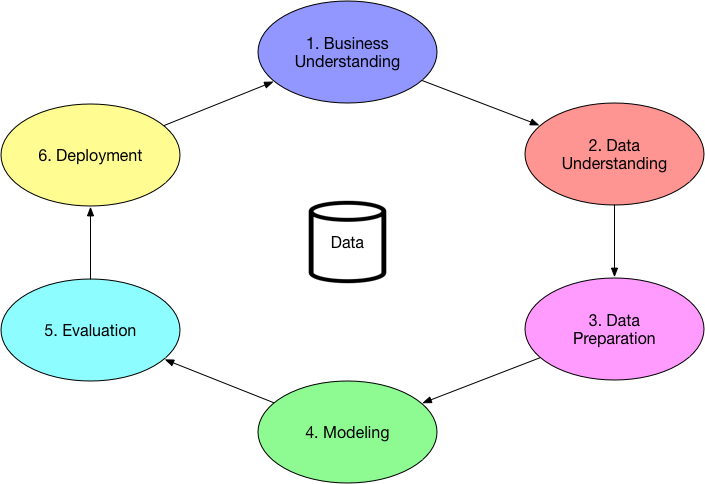
\includegraphics[width=\textwidth]{gfx/CRISP-DM_Model.png}
	\caption{Konzeptionelles CRISP-DM Modell}
	\label{fig:process:crispdm}
\end{figure}

\subsection{Business Understanding}
\label{sec:process:crispdm:bu}

Im ersten Schritt des CRISP-DM Prozesses, dem sog. Business- (oder auch Organizational-) Understanding,
ist es zunächst wichtig festzulegen was man mit dem Minen von Daten erreichen
möchte bzw. welche Informationen von Interesse sind. Hier findet auch eine oft
zitierte Textstelle aus Alice im Wunderland Anwendung:
\begin{quotation}
  >>Willst du mir wohl sagen, wenn ich bitten darf, welchen Weg ich hier nehmen muß?<< \\
  >>Das hängt zum guten Teil davon ab, wohin du gehen willst,<< sagte die Katze. \\
  >>Es kommt mir nicht darauf an, wohin –<< sagte Alice. \\
  >>Dann kommt es auch nicht darauf an, welchen Weg du nimmst,<< sagte die Katze. \\
  >>– wenn ich nur irgendwo hinkomme,<< fügte Alice als Erklärung hinzu. \\
  >>O, das wirst du ganz gewiß,« sagte die Katze, »wenn du nur lange genug gehest.<<
\end{quotation}
Konkret bedeutet das, dass es keine Rolle spielt wie lange man Daten Mined, wenn
man nicht festgelegt hat welche Informationen man gerne hätte. Es müssen also
zunächst Fragen festgelegt werden, welche durch das Data Mining beantwortet
werden sollen. Beispielsweise möchte man gerne wissen warum sich Kunden so sehr
beschweren, wie man die Profit-Spanne seiner Produkte vergrößert oder wie man
Fehler bei der Herstellung antizipieren kann.

\subsection{Data Understanding}
\label{sec:process:crispdm:du}



\subsection{Data Preparation}
\label{sec:process:crispdm:dp}

\subsection{Modeling}
\label{sec:process:crispdm:mod}

\subsection{Evaluation}
\label{sec:process:crispdm:eval}

\subsection{Deployment}
\label{sec:process:crispdm:depl}

\section{Alternativen}
\label{sec:alt}

% !TEX root = ../Seminararbeit-Data_Mining_Frameworks.tex
%


% =============================================================================
%
% Vorsstellung der Software
%
% =============================================================================
\chapter{Vorstellung der Software}
\label{sec:software}

\section{Rapidminer Studio}
\label{sec:software:rm}

Bei RapidMiner handelt es sich um eine „Open Source Data Science Platform“,
welche vom gleichnamigen Unternehmen unter der AGPL 3.0 Lizenz vertrieben wird.
Der Quellcode ist offen und kann auf Github gefunden werden. Neben dem im
Folgenden näher untersuchten „RapidMiner Studio“ bietet die Plattform noch die
Produkte „RapidMiner Server“ zur Automatisierung von Prozessen und „RapidMiner
Radoop“ welches es erlaubt Berechnungen in einer Hadoop Umgebung auf einem
Cluster auszuführen. Für kleinere Datensätze mit bis zu 10.000 Einträgen steht
eine kostenlose „Education Version“ zur Verfügung. Außerdem bietet der
Hersteller die Software für sämtliche Plattformen (Windows, MacOS, Linux) an. \\
Das Tool „RapidMiner Studio“ bietet die Möglichkeit einen
Datenverarbeitungsprozess mithilfe einer eingängigen Oberfläche zu erstellen.
Dafür muss die Software zunächst (auf einer der oben genannten Plattformen)
installiert werden.

\begin{figure}[htb]
	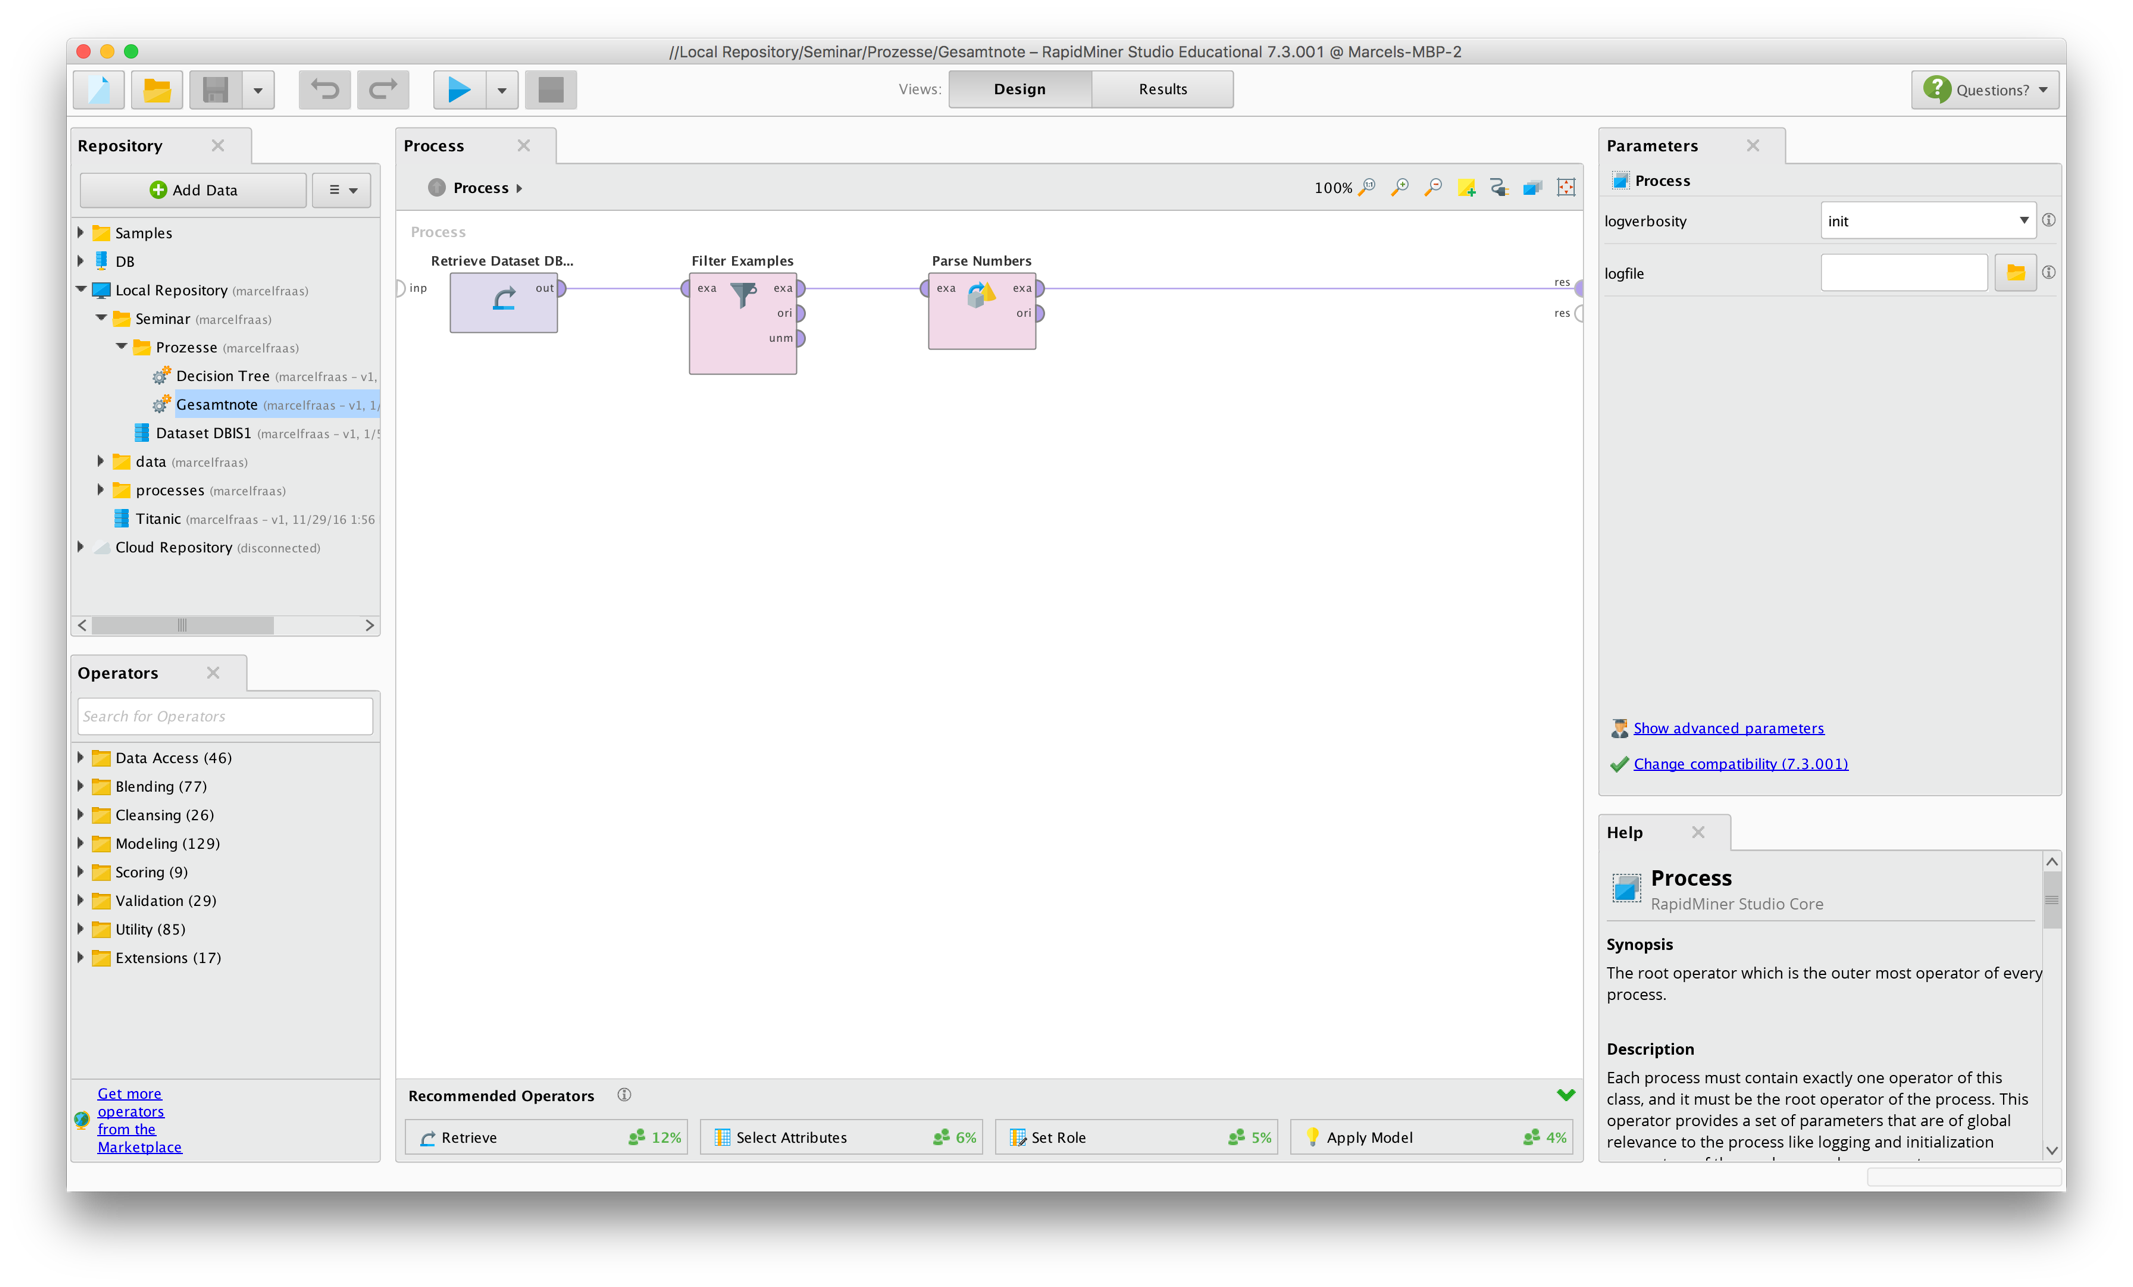
\includegraphics[width=\textwidth]{gfx/rm1.png}
	\caption{Die RapidMiner Design View}
	\label{fig:software:rm:des}
\end{figure}

Die Oberfläche bietet ein Intuitives User Interface, welches die Einarbeitung
sehr vereinfacht. Im Abschnitt links oben befindet sich das sog. „Repository“.
Hier befinden sich die konfigurierten Datenquellen, welche bspw. in Form von
Excel-, Access-, SAS oder SPSS Dateien vorliegen können. Alternativ können auch
direkt SQL Datenbanken, wie MySQL, Microsoft SQL Server, Oracle, PostgreSQL
u.a., angebunden werden. \\
Darunter befindet sich die Ordnerstruktur der „Operators“. Von hier können die
zahlreichen Operatoren per Drag and Drop in den Hauptbereich der Design-Ansicht,
dem sog. „Process“ gezogen werden. \\
In der Prozessübersicht können Operatoren und Repositories angeordnet und
miteinander verknüpft werden. \\
Auf der rechten Seite befinden sich, neben der Hilfe, noch eine Übersicht über
die Parameter des aktuell ausgewählten Operators. \\
Zu guter Letzt bietet RapidMiner Studio noch eine zusätzliche Hilfsfunktion,
die sog. „Recommended Operators“. Hier werden mit Hilfe von statistischen
Auswertungen die am wahrscheinlichsten, zum aktuellen Prozess passenden,
nächsten Operatoren angezeigt. Dies erleichtert den Einstieg in die Software ungemein.

\begin{figure}[htb]
	%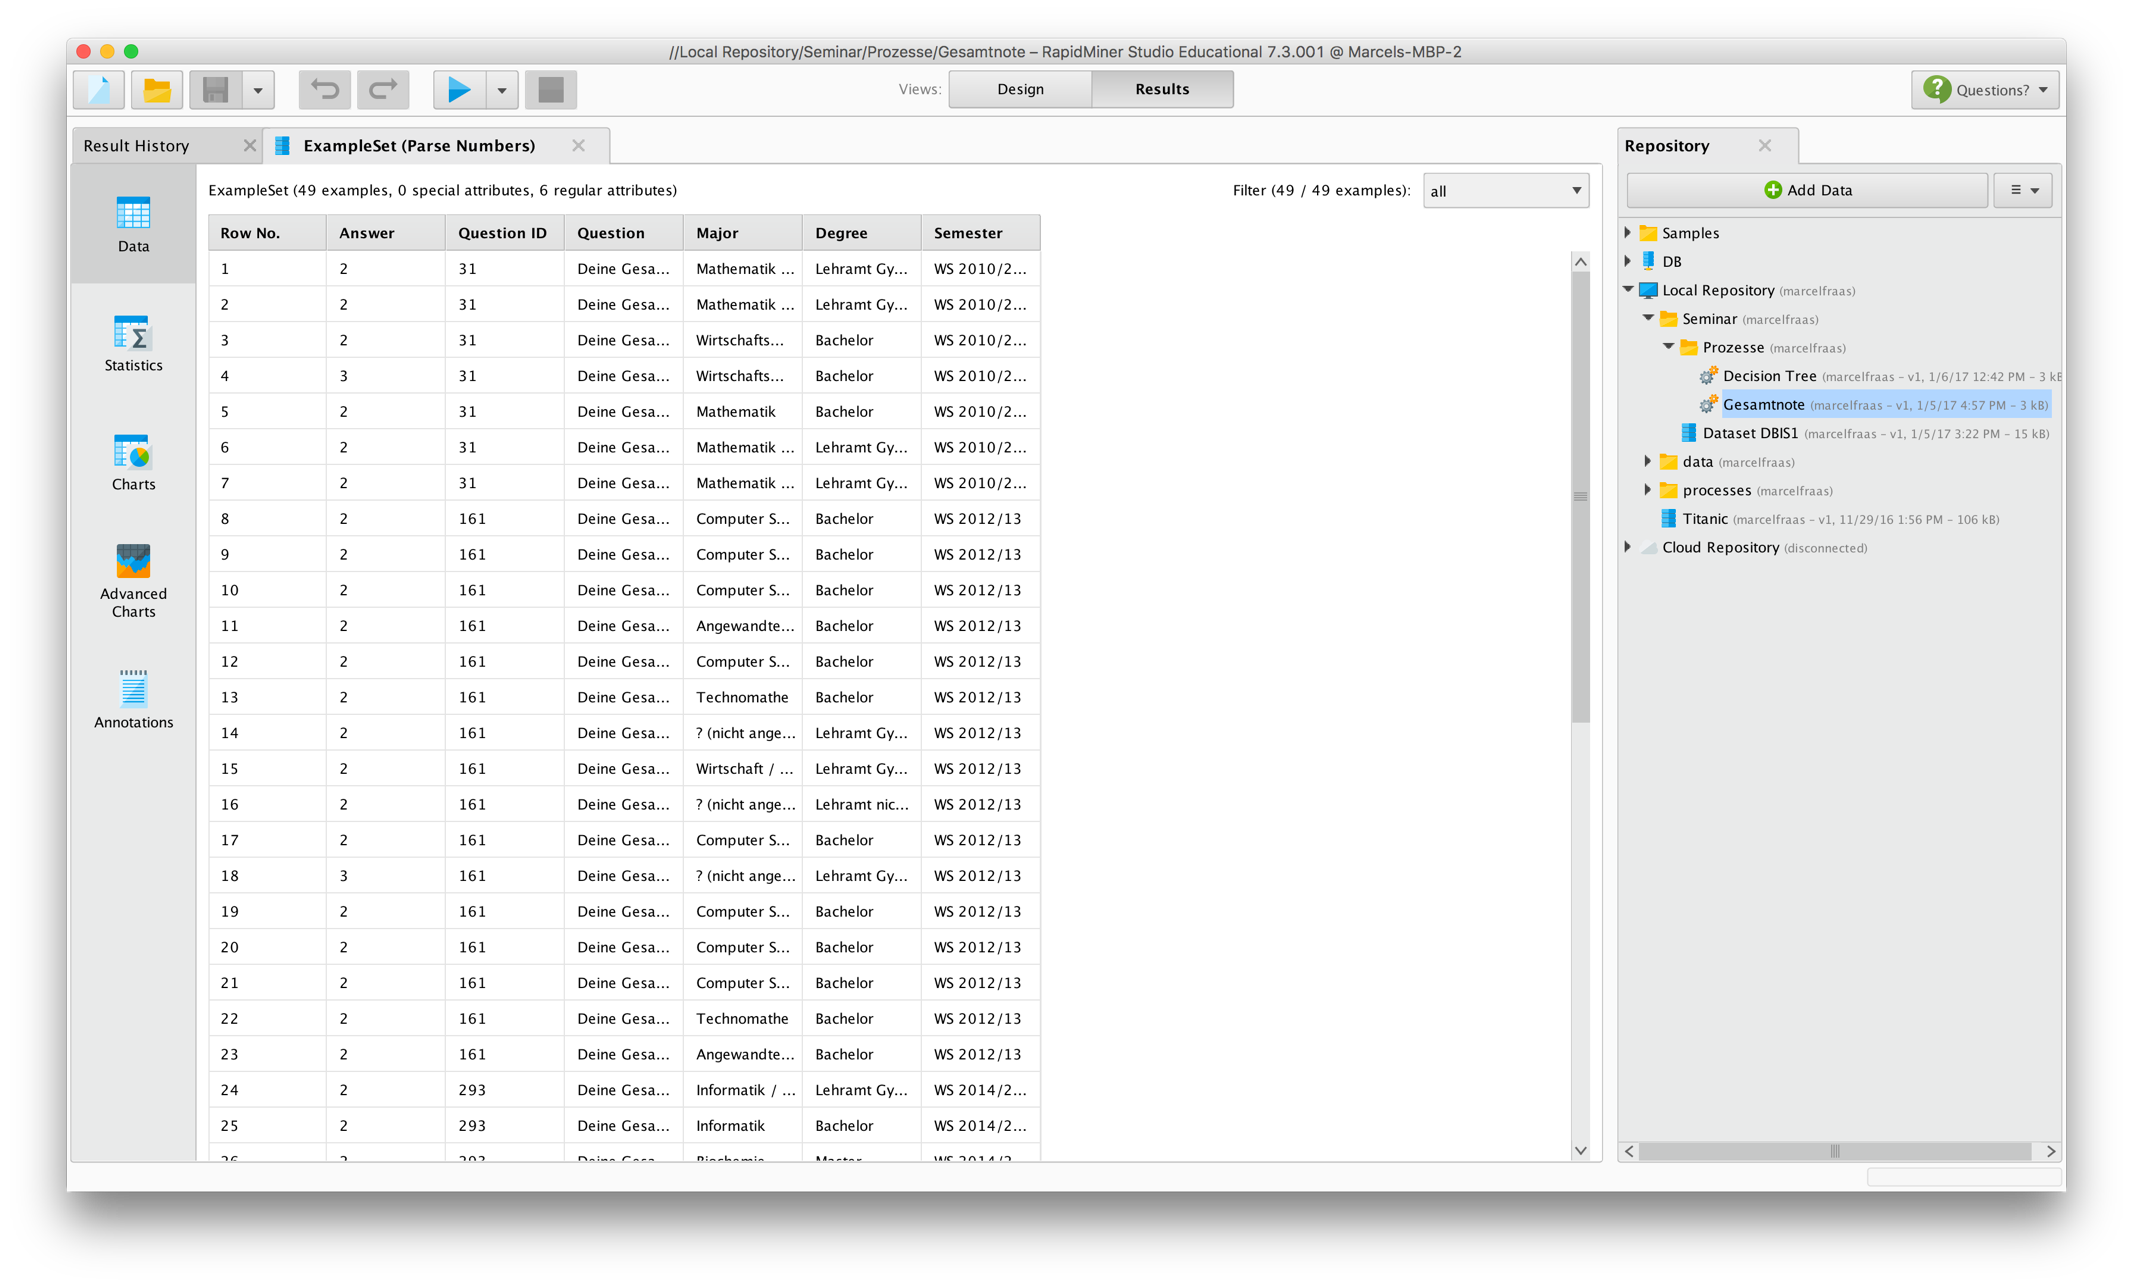
\includegraphics[width=\textwidth]{gfx/rm2.png}
  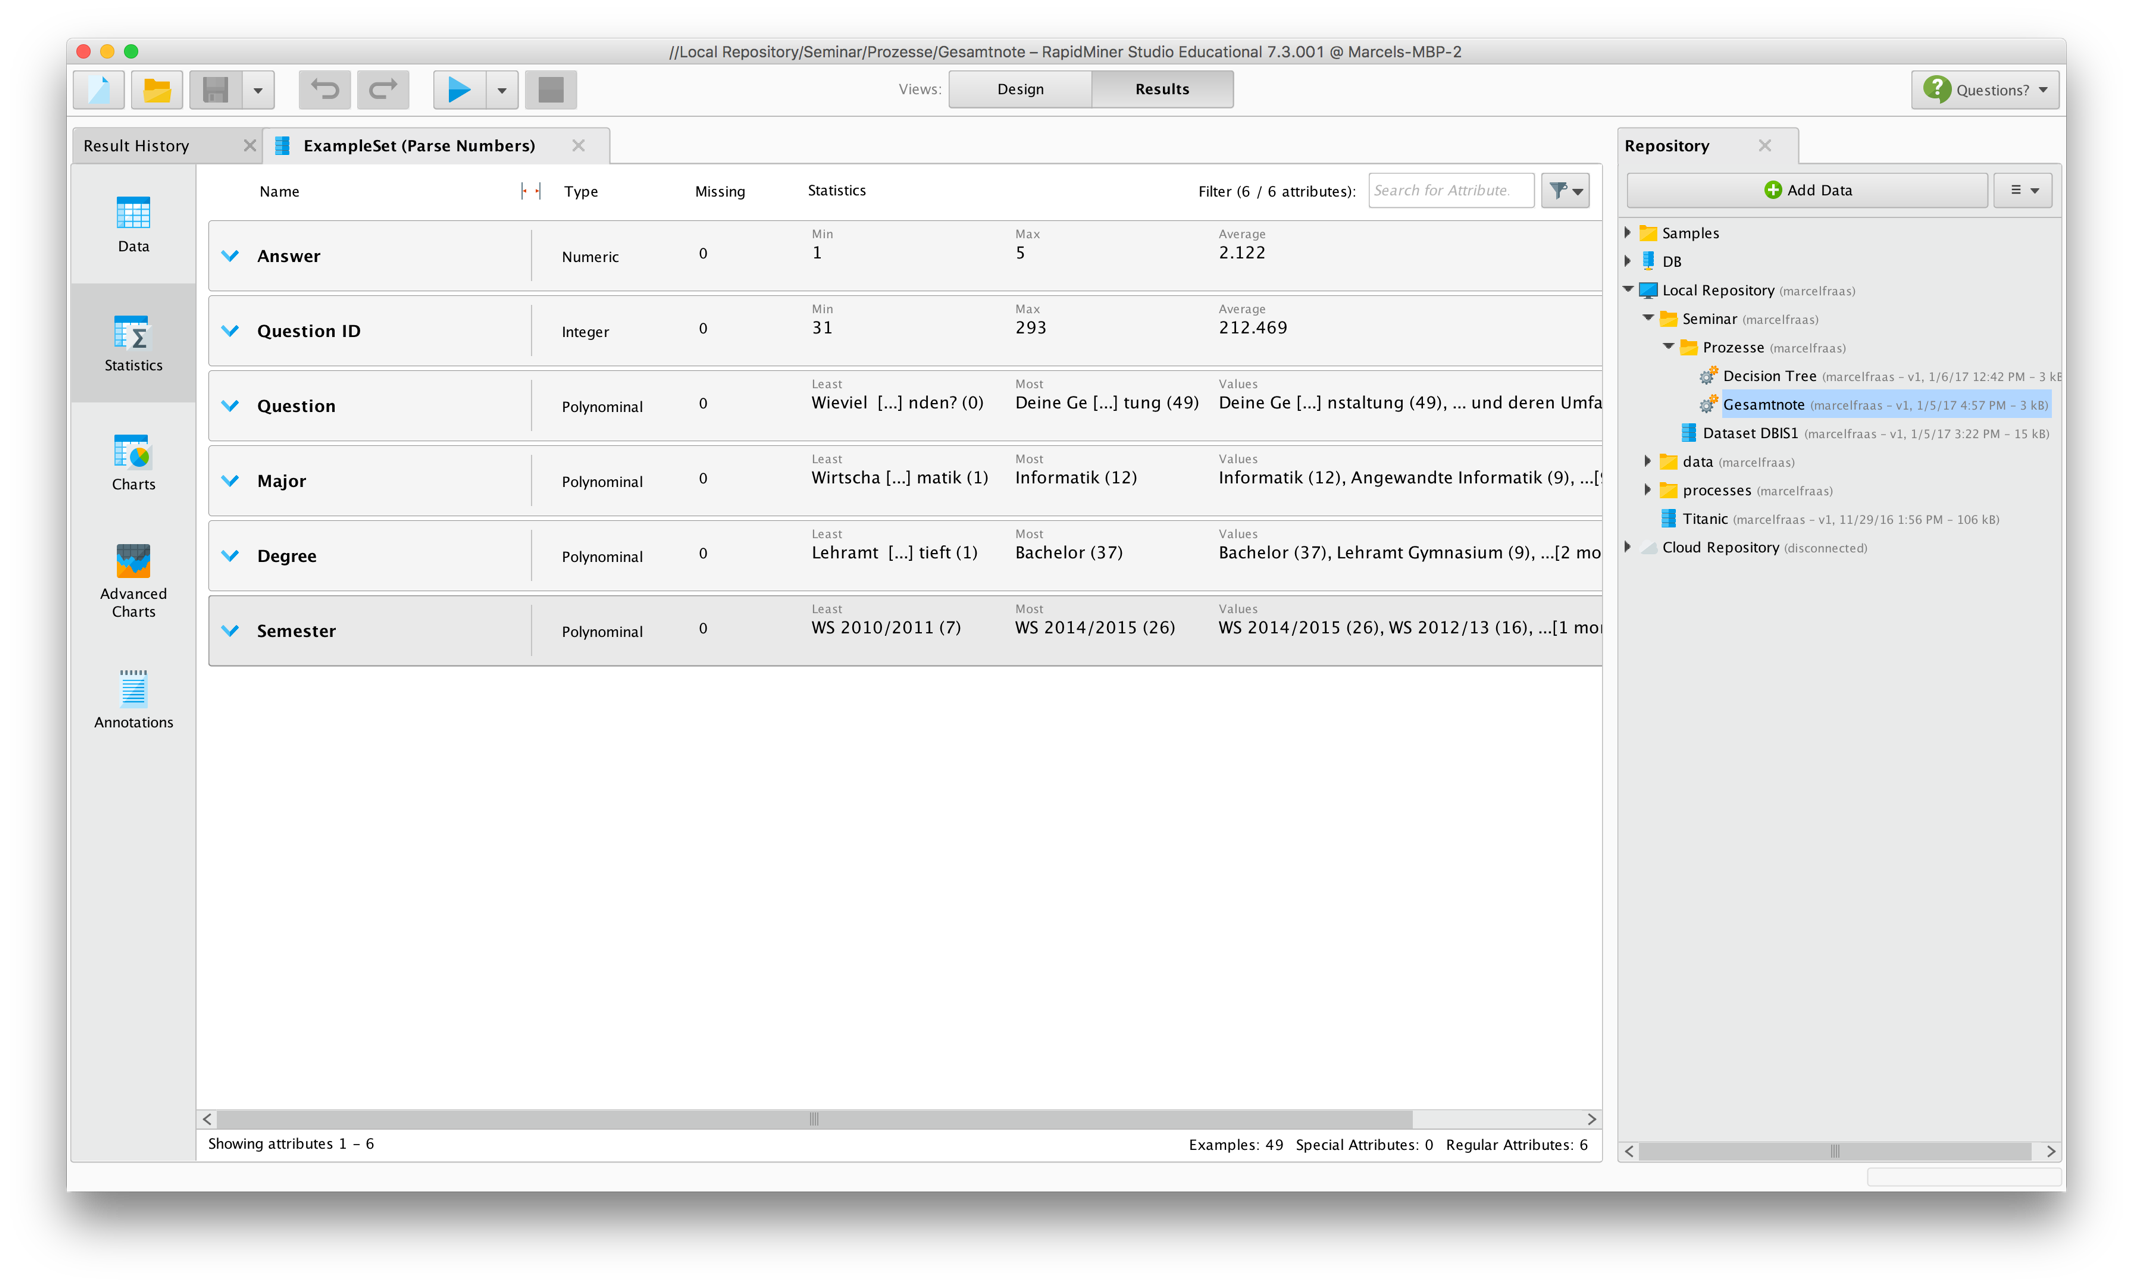
\includegraphics[width=\textwidth]{gfx/rm3.png}
	\caption{Die RapidMiner Result View}
	\label{fig:software:rm:res}
\end{figure}

Führt man einen Prozess aus, bzw. wählt man manuell in der Menüleiste den Reiter
„Results“ bekommt man das Ergebnis entweder in roh Form, also als Tabelle, in
einer statistischen Übersicht oder als Graph bzw. Diagramm.


Generell ist die Einarbeitung in RapidMiner Studio, gerade auch wegen den
detaillierten Hilfsfunktionen, sehr eingängig und führt schnell zu Ergebnissen.

\pagebreak

\section{Microsoft Azure Machine Learning Studio}
\label{sec:software:msa}

Das „Microsoft Azure Machine Learning Studio“ ist, wie der Name bereits verrät,
teil der Microsoft Cloud Umgebung Azure. Folglich ist das Tool eine Webanwendung,
welche per Browser gestartet werden kann.  Für den Einstieg benötigt man
lediglich einen Microsoft Azure Account, welchen man kostenlos erstellen kann.
Damit hat man dann vollen Zugriff auf alle Funktionen des Machine Learning
Studios. Einschränkungen des kostenlosen Accounts gibt es hier nur bezüglich
der Rechenzeit und den weiteren Services der Azure Umgebung (APIs etc.). \\
Neben dem Machine Learning Studio bietet die Microsoft Cloud eine Vielzahl an
Services und Ressourcen, wie virtualisierte Server, Hosting von Webanwendungen
und APIs sowie Datenbanken. Durch den „Platform as a Service“ Aspekt, wird eine
extrem einfache Kollaboration und schnelles Deployment ohne eigenen
Administrationsaufwand gewährleistet.

\begin{figure}[htb]
	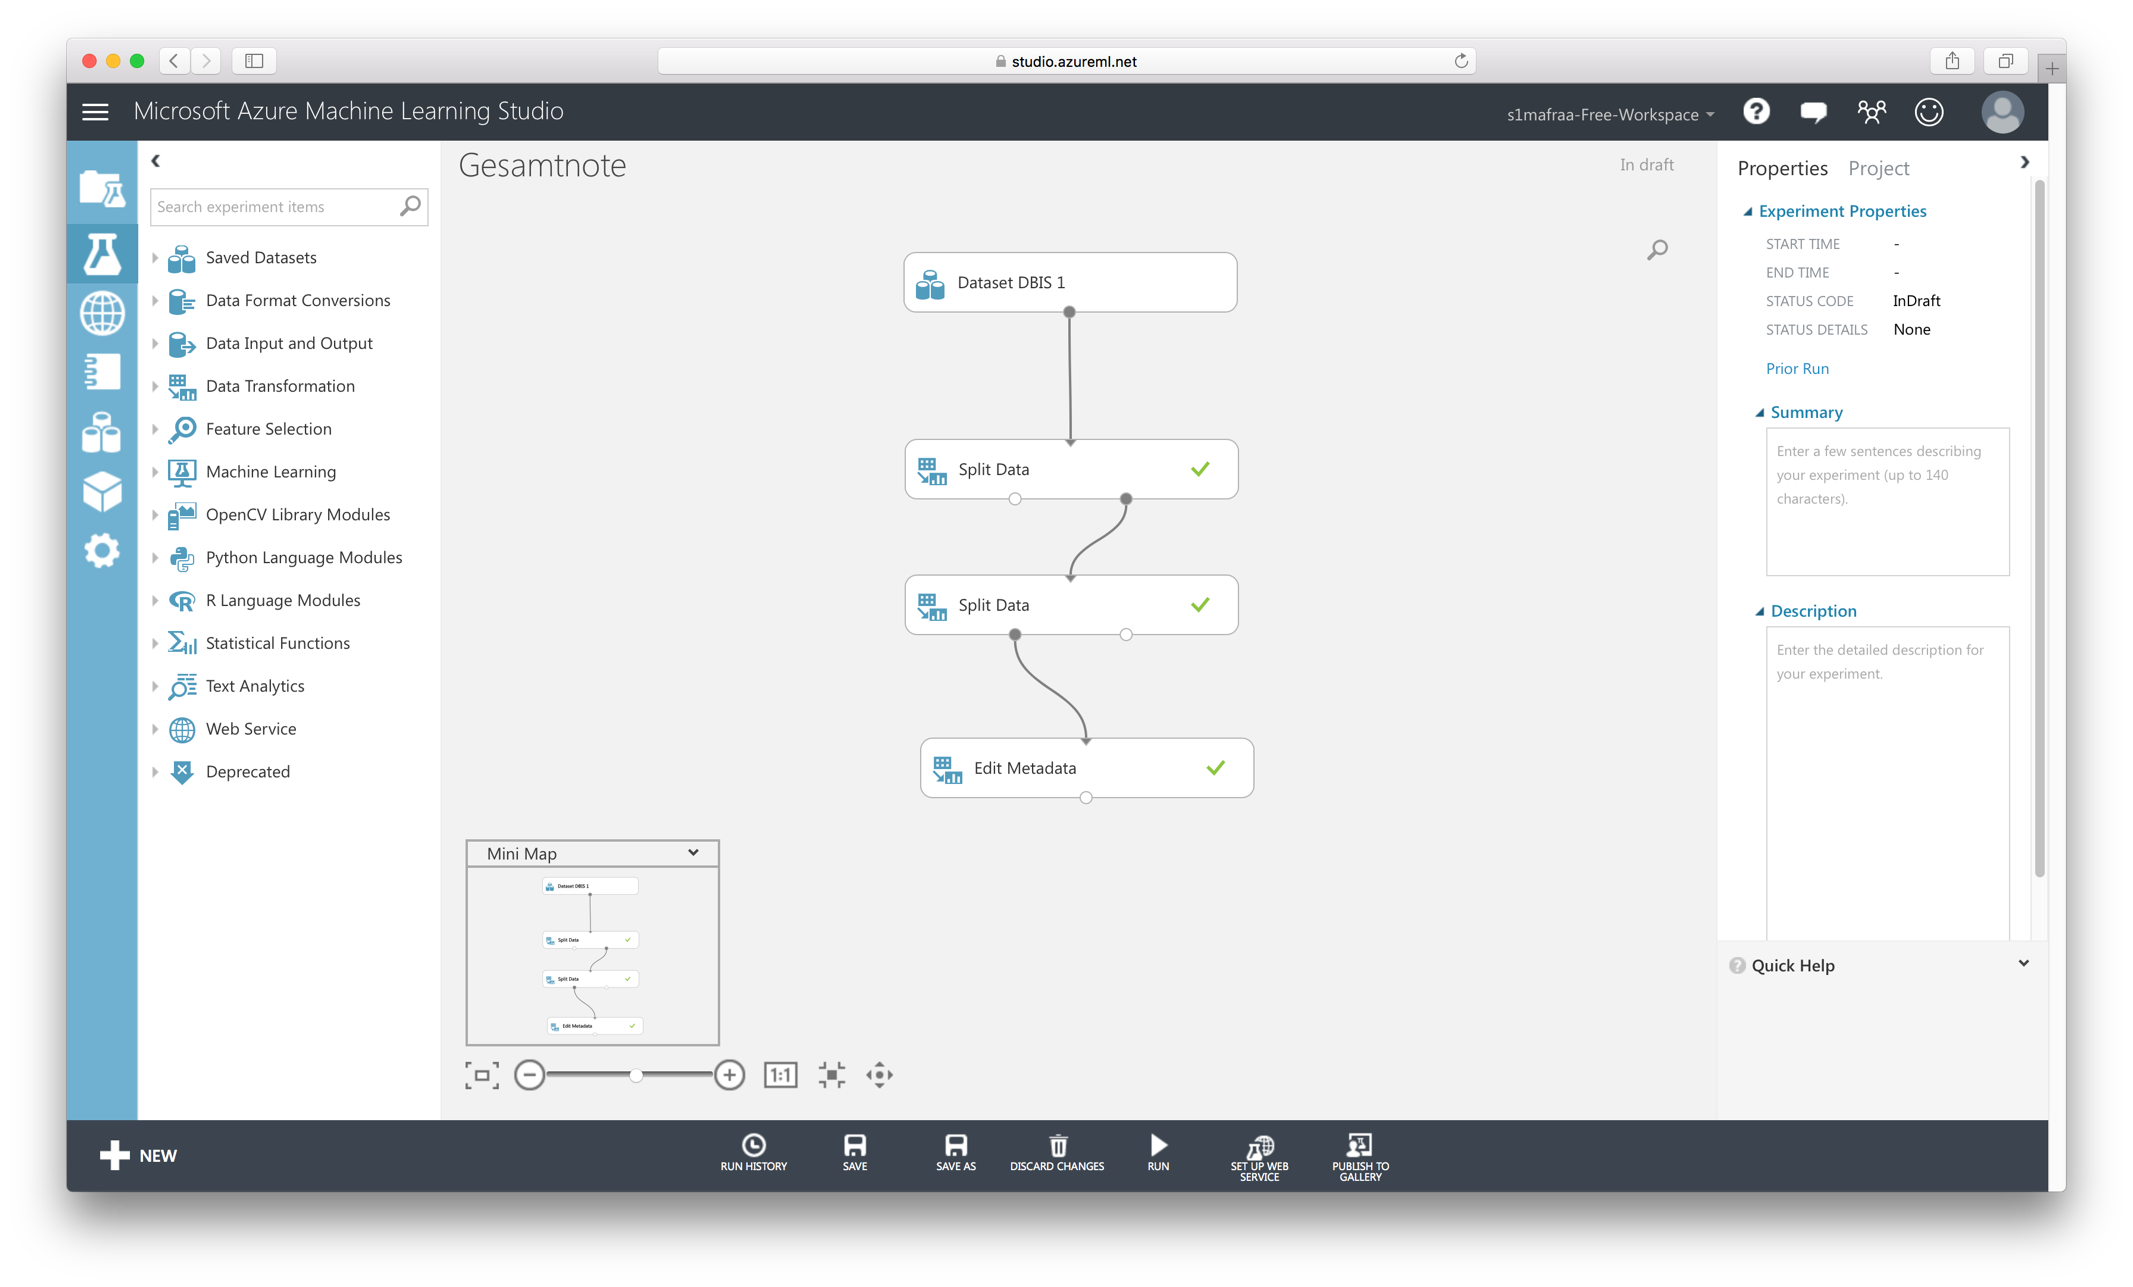
\includegraphics[width=\textwidth]{gfx/ml1.png}
	\caption{Ein Expriment im MSA Machine Learning Studio}
	\label{fig:software:ml:des}
\end{figure}

Nach dem starten der Webanwendung kann der Anwender direkt damit beginnen ein
neues Experiment anzulegen. Die Oberfläche ist ähnlich dem RapidMiner User
Interface aufgebaut. Auf der linken Seite befinden sich die Datenquellen und
die Operatoren. Unterstützt werden von Microsoft u.a. die Excel-, CSV-, ARFF-,
sowie Plain Text und RObject Dateiformate. Außerdem können natürlich ebenfalls
Daten aus einer SQL Datenbank, wie beispielsweise einer Microsoft SQL
Serverinstanz aus der Azure Cloud, geladen werden. \\
Auch hier können die Operatoren per Drag and Drop in die Arbeitsfläche gezogen
werden und mit den Parametern am rechten Rand konfiguriert werden.

\begin{figure}[htb]
	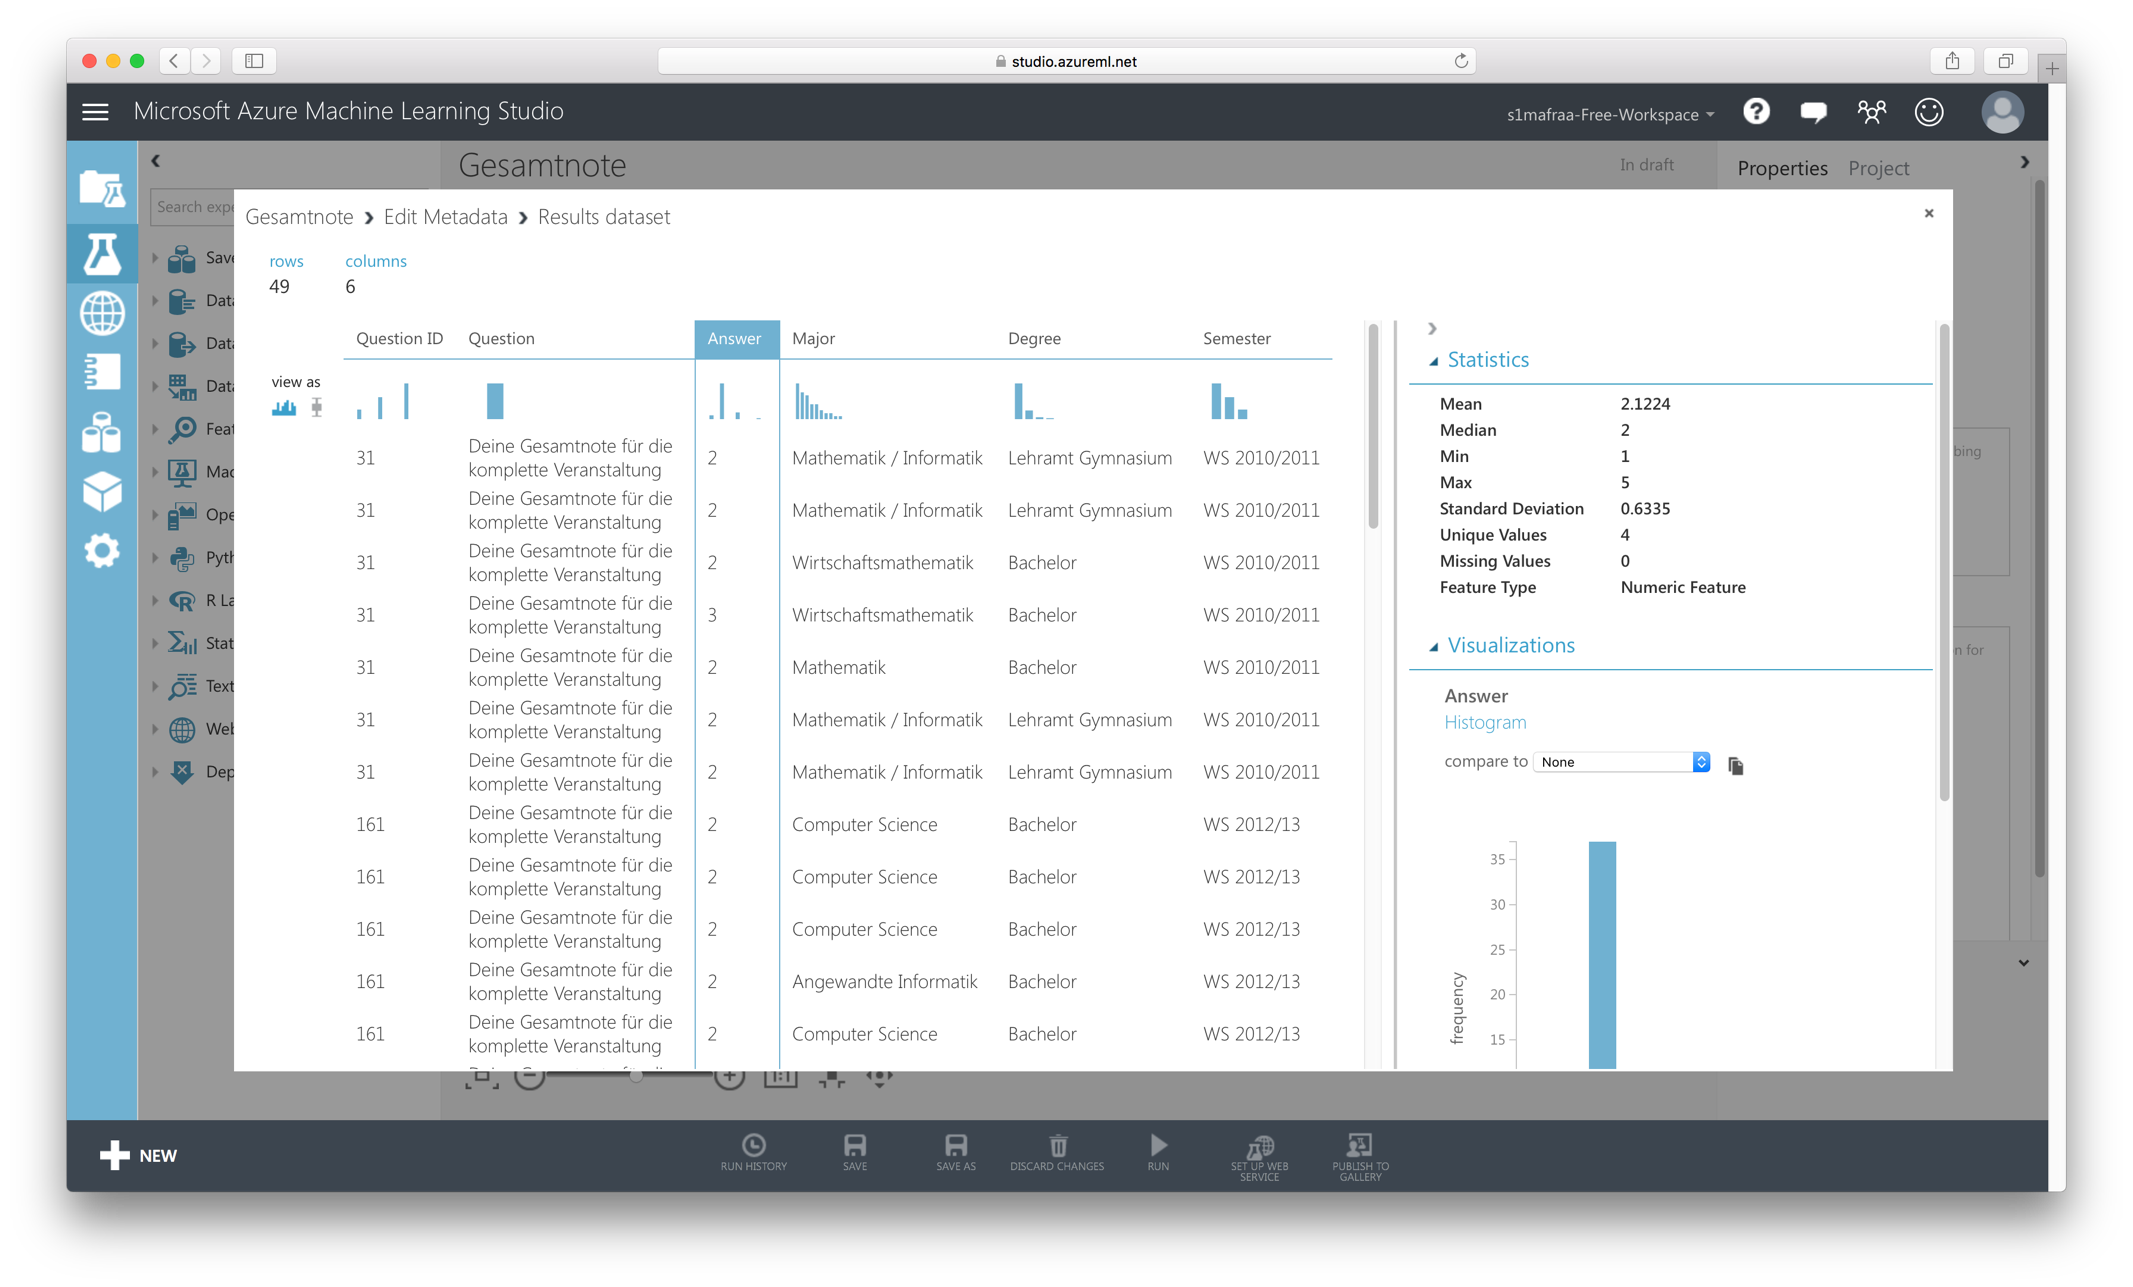
\includegraphics[width=\textwidth]{gfx/ml2.png}
	\caption{Das Ergebnis eines Expriments im MSA Machine Learning Studio}
	\label{fig:software:ml:res}
\end{figure}

Die Visualisierung des Ergebnisses ist im Machine Learning Studio abhängig vom
jeweiligen Experiment. In diesem Fall wird dieses als Tabelle mit einigen
Statistiken und Diagrammen dargestellt.


Aufgrund der Tatsache, dass es sich beim Microsoft Azure Machine Learning Studio
um eine Webanwendung handelt, müssen ein paar Abstriche in Sachen Bedienbarkeit
gemacht werden. Dafür ist die Kollaboration mit Anderen und die Einbindung in
Webservices erheblich vereinfacht, was besonders zum Tragen kommt, wenn man
bereits eine gewisse Infrastruktur innerhalb der Azure Cloud besitzt.

% !TEX root = ../Seminararbeit-Data_Mining_Frameworks.tex
%


% =============================================================================
%
% Datensatz und Beispiel-Modell
%
% =============================================================================
\chapter{Datensatz und Beispiel-Modell}
\label{sec:example}

\section{Datensatz}
\label{sec:example:data}

\begin{figure}[htb]
	
\includegraphics[width=\textwidth]{gfx/crisplinear.png}
	\caption{Der CRISP-DM Prozess als Kette der einzelnen Schritte}
	\label{fig:example:data:crisp}
\end{figure}

Für die Umsetzung des Beispiels wurde der Eingangs bereits beschriebene CRISP-DM
Data Mining Prozess verwendet. Die Daten wurden gemäß den 6 Schritten „Business
Understanding“, „Data Understanding“, „Data Preparation“, „Modeling“,
„Evaluation“ und „Deployment“ verarbeitet.

\subsection{Business Understanding}
\label{sec:example:data:bu}

Als Datengrundlage für das Beispiel dienen die Daten der
Veranstaltungsevaluationen der Vergangenen Semester, durchgeführt von der
Fachschaft Mathematik, Physik und Informatik der Universität Bayreuth. Mithilfe
der vorliegenden Datengrundlage sollen nun folgende Fragen beantwortet werden:

\begin{itemize}
  \item „Warum beschweren sich einige Studenten, während andere die Veranstaltung
  super finden? Bzw. welche Ursachen gibt es für eine Beschwerde?“
  \item „Wie sind die Prognosen für die bevorstehenden Evaluationen?“
\end{itemize}

\subsection{Data Understanding}
\label{sec:example:data:du}

Im nächsten Schritt ist es wichtig herauszufinden, wie die Daten erhoben wurden.
Im Beispiel der Veranstaltungsevaluationen ist dies durch Austeilen eines
Fragebogens erfolgt.

\begin{figure}[htb]
	
\includegraphics[width=\textwidth]{gfx/questionnaire.png}
	\caption{Fragebogen, zur Erhebung der Evaluationsdaten}
	\label{fig:example:data:du:qu}
\end{figure}

Anhand des Fragebogens erkennt man, dass die Antwortmöglichkeiten in Form von
anzukreuzenden Kästchen gegeben waren. Jedes Kreuz repräsentiert dabei einen
Wert im Bereich von 0 bis max. 4. \\
Außerdem muss festgestellt werden, wie die Daten in der Datenbank abgelegt
werden. Hierfür kann man bspw. ein ER-Diagramm erzeugen oder sich eine Vorschau
der Daten in Form einer Tabelle generieren lassen.

\begin{figure}[htb]
  \center
	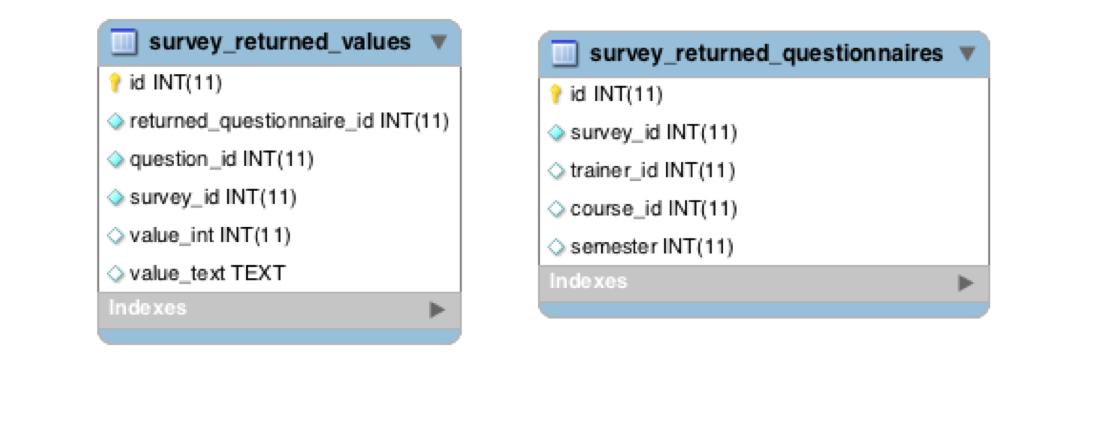
\includegraphics[width=0.7\textwidth]{gfx/db1.png}
  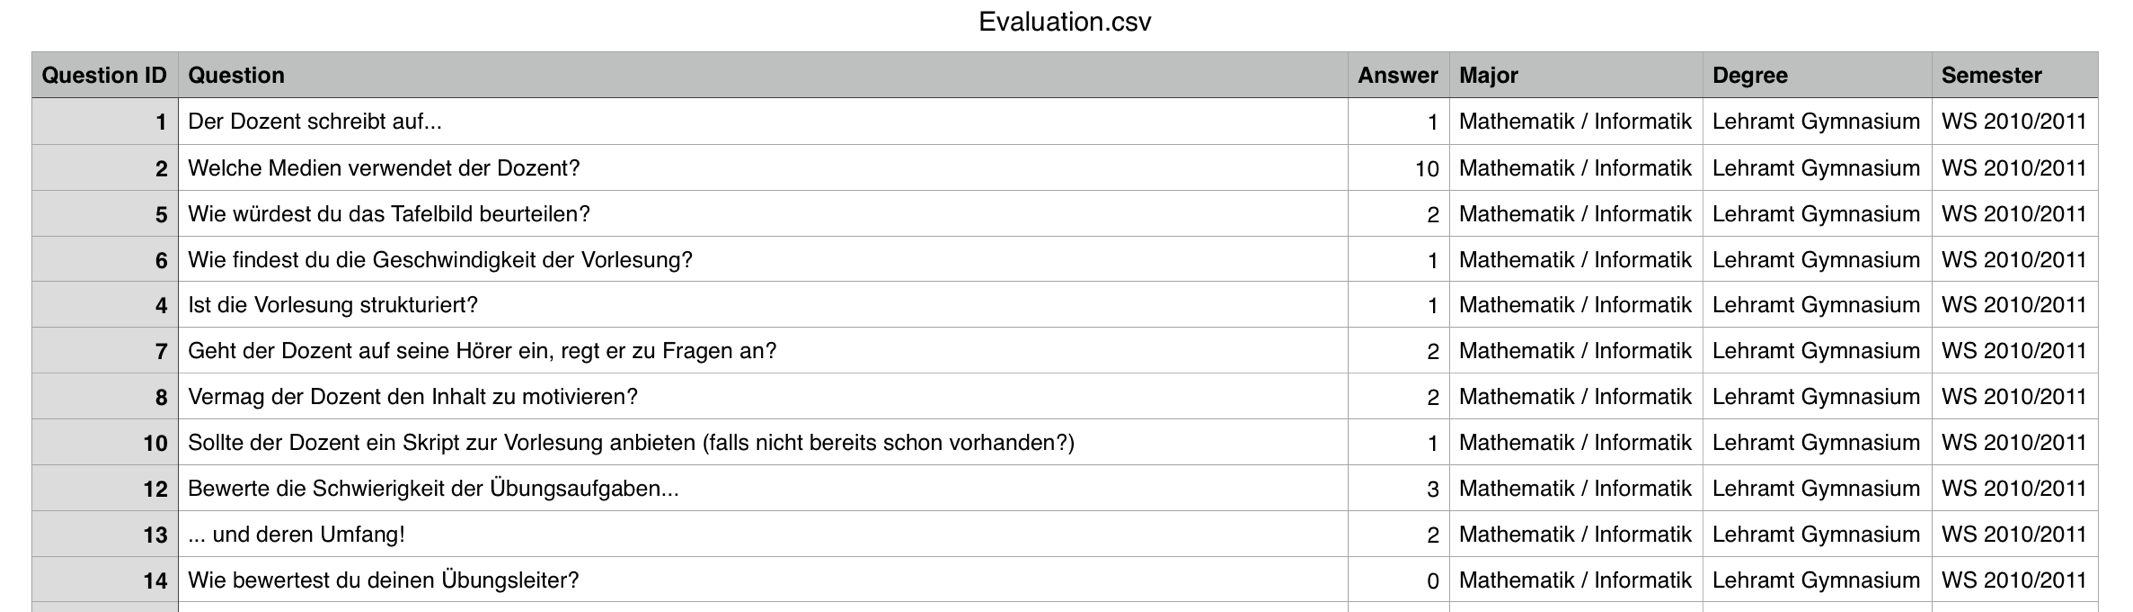
\includegraphics[width=\textwidth]{gfx/db2.png}
	\caption{Repräsentation der Daten in der Datenbank}
	\label{fig:example:data:du:db}
\end{figure}

Mithilfe dieser Informationen erkennt man, dass sich die gesuchten Daten in den
beiden Tabellen „survey\_returned\_values“ und „survey\_returned\_questionnaires“
befinden und wie diese strukturiert sind.

\subsection{Data Preparation}
\label{sec:example:data:dp}

Wurden nun die entsprechenden Tabellen bzw. deren Attribute festgelegt, müssen
diese nun im nächsten Schritt aus der Datenbank extrahiert werden, um separat
Analysiert werden zu können. Dies geschieht mit der folgenden SQL-Abfrage.

\begin{figure}[htb]
	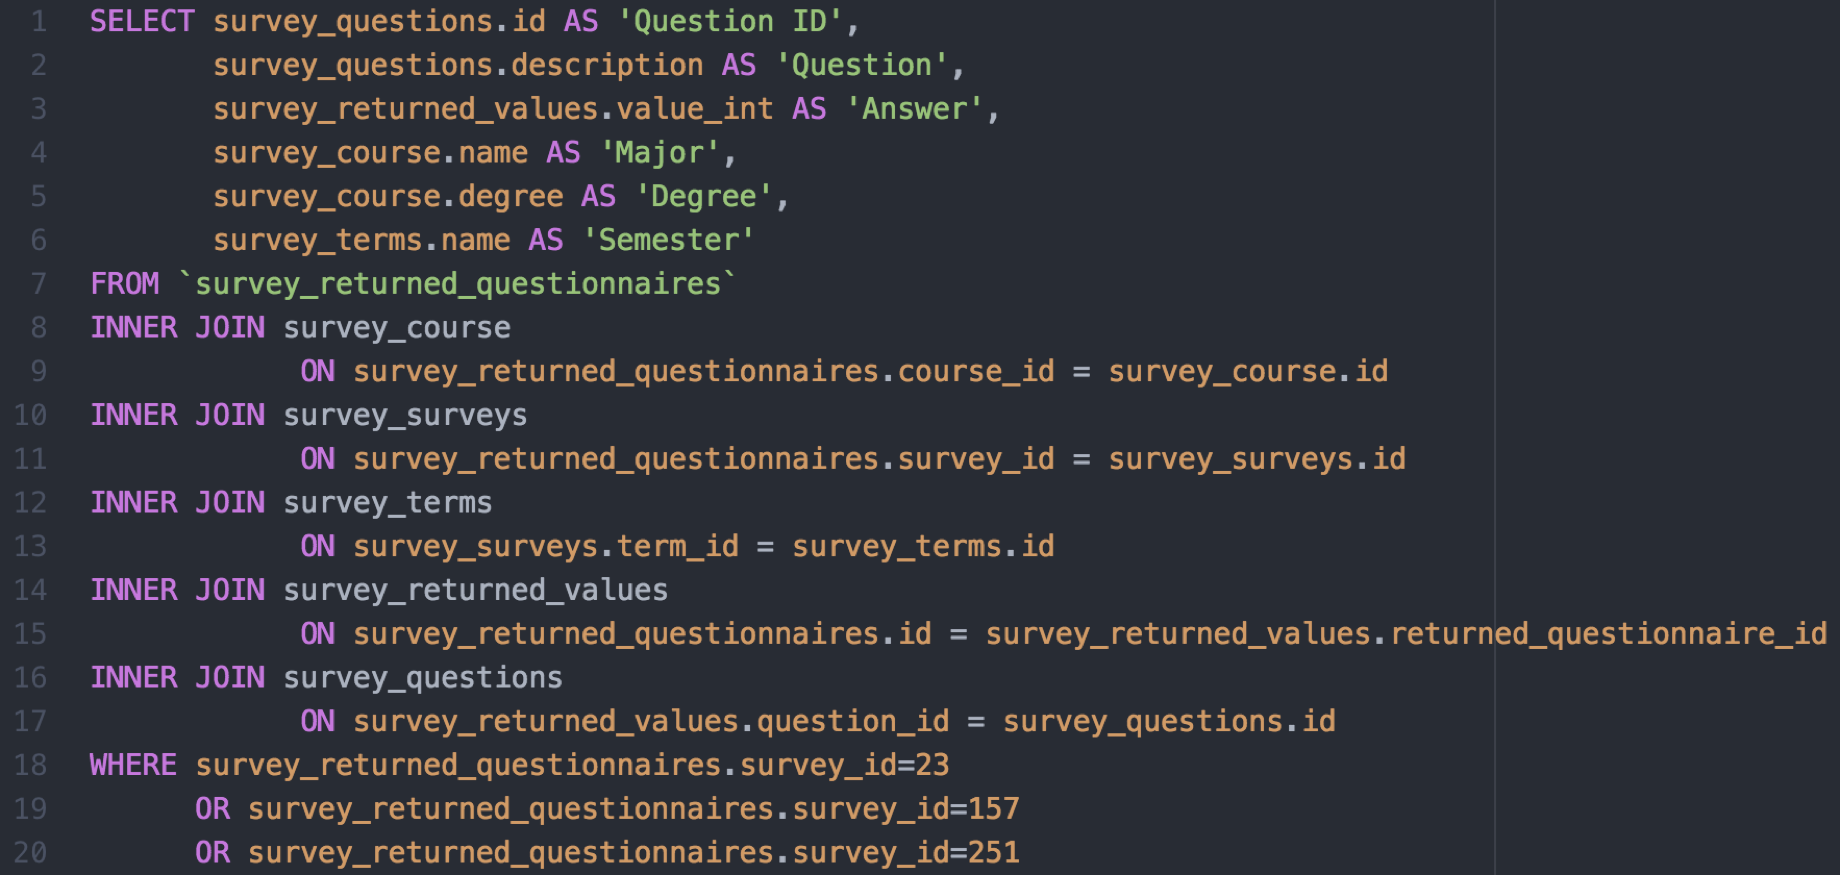
\includegraphics[width=\textwidth]{gfx/sql.png}
	\caption{SQL Anfrage für den Export der Daten}
	\label{fig:example:data:dp:sql}
\end{figure}

Die Ergebnisdatensätze der SQL-Abfrage können nun als .csv Datei exportiert
werden, um danach in der jeweiligen Data Mining Software verarbeitet werden zu
können.

\subsection{Modeling}
\label{sec:example:data:mod}

In der Modellierungsphase muss nun ein Algorithmus gewählt werden, welcher die
vorbereiteten Daten so verarbeiten kann, dass die definierten
Fragestellungen beantwortet werden können. In unserem Beispiel eignet sich die
Frage nach der Gesamtnote, da dieses Attribut eine gute Repräsentation der
Gesamtbewertung für eine Veranstaltung darstellt. \\
Es muss also ein Algorithmus gewählt werden, welcher nach einem einzelnen
Attribut, dem sog. Label, Daten Mined. Ein einfach auszuwertender Algorithmus,
der genau diese Voraussetzungen erfüllt ist der sog. „Entscheidungsbaum“
(engl.: „Decision Tree“).

\begin{figure}[htb]
  \center
	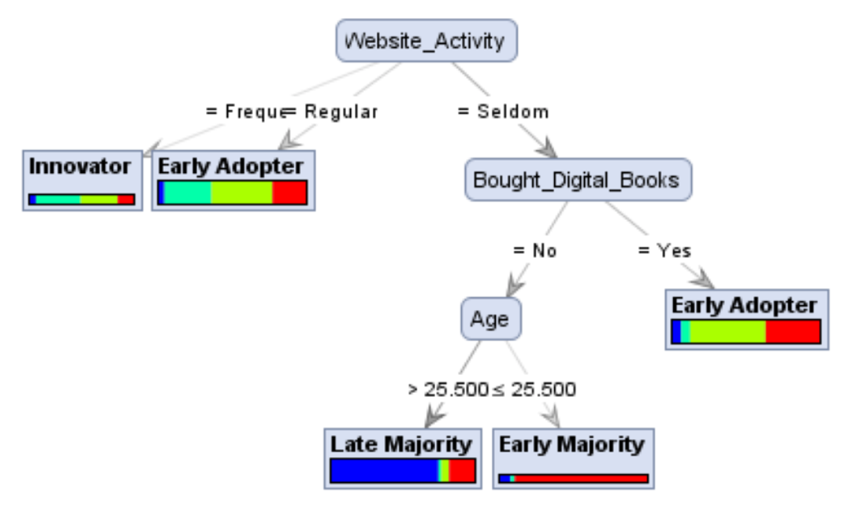
\includegraphics[width=0.5\textwidth]{gfx/dt.png}
	\caption{Beispiel für einen Entscheidungsbaum \cite{North:2012}}
	\label{fig:example:data:mod:dt}
\end{figure}

Die Knoten des Baumes stellen klassifizierende Attribute des Ausgangs-Datensatzes
dar, während die Blätter die möglichen Werte des Labels anzeigen. Außerdem
zeigen die Blätter noch an, auf wieviel Datensätzen die jeweilige Klasse beruht.

\subsection{Evaluation + Deployment}
\label{sec:example:data:eval}

Schließlich kann mithilfe des „Decision Trees“ ermittelt werden, dass
beispielsweise das Studienfach oder ein bestimmtes Semester die Ursache für
vermehrte Beschwerden (respektive mehrere schlechte Bewertungen) waren.
Gleichzeitig kann man mit den entsprechenden Informationen über Studienfach,
Abschluss etc. der aktuellen Kursteilnehmer eine Prognose für die bevorstehende
Lehrveranstaltungsevaluation abgeben.

\section{Umsetzung}
\label{sec:example:impl}

\subsection{Rapidminer Studio}
\label{sec:example:impl:rm}

Um das Beispielszenario in RapidMiner Studio umzusetzen wurde der folgende
Prozess modelliert:

\begin{figure}[htb]
  \center
	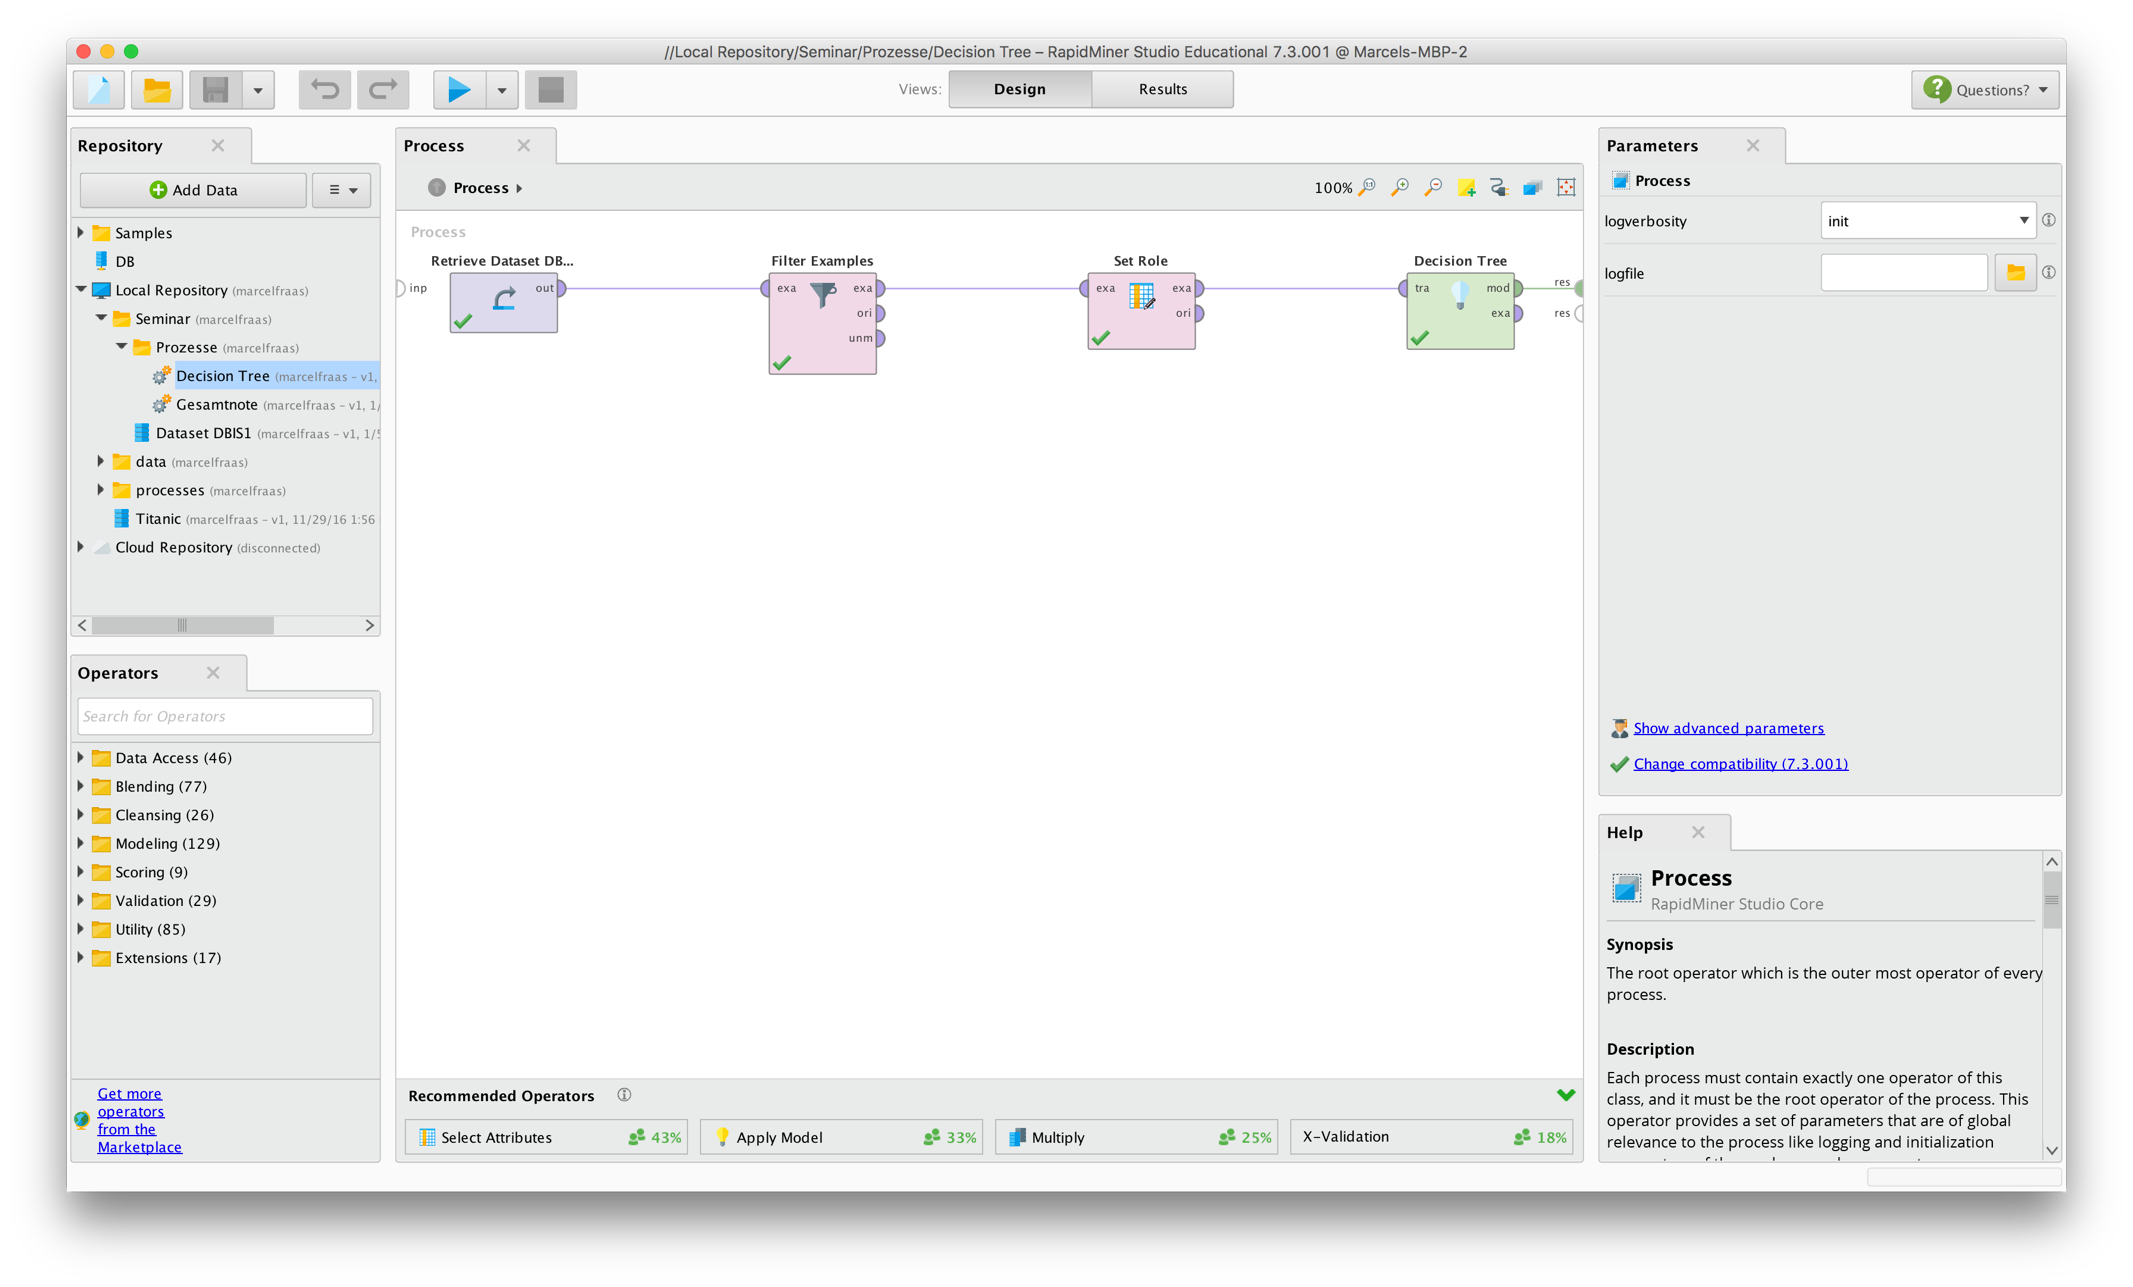
\includegraphics[width=0.9\textwidth]{gfx/rmproc.png}
	\caption{Der Beispielprozess im RapidMiner Studio}
	\label{fig:example:impl:rm:proc}
\end{figure}

Zunächst wurde die .csv Datei mit dem „Retrieve Dataset“ Operator in den Prozess
geladen. Anschließend wurden per „Filter Example“ sowohl alle Datensätze mit
NULL Einträgen entfernt, als auch die Einträge, welche die Frage nach der
Gesamtnote beinhalten, extrahiert. Danach wurde die Spalte „Answer“, welche den
Wert der Note beinhaltet als „Label“ definiert. Zuletzt wurden die Daten dann
dem „Decision Tree“ Algorithmus übergeben und das Ergebnis zurück in die Anzeige
geladen.

\begin{figure}[htb]
	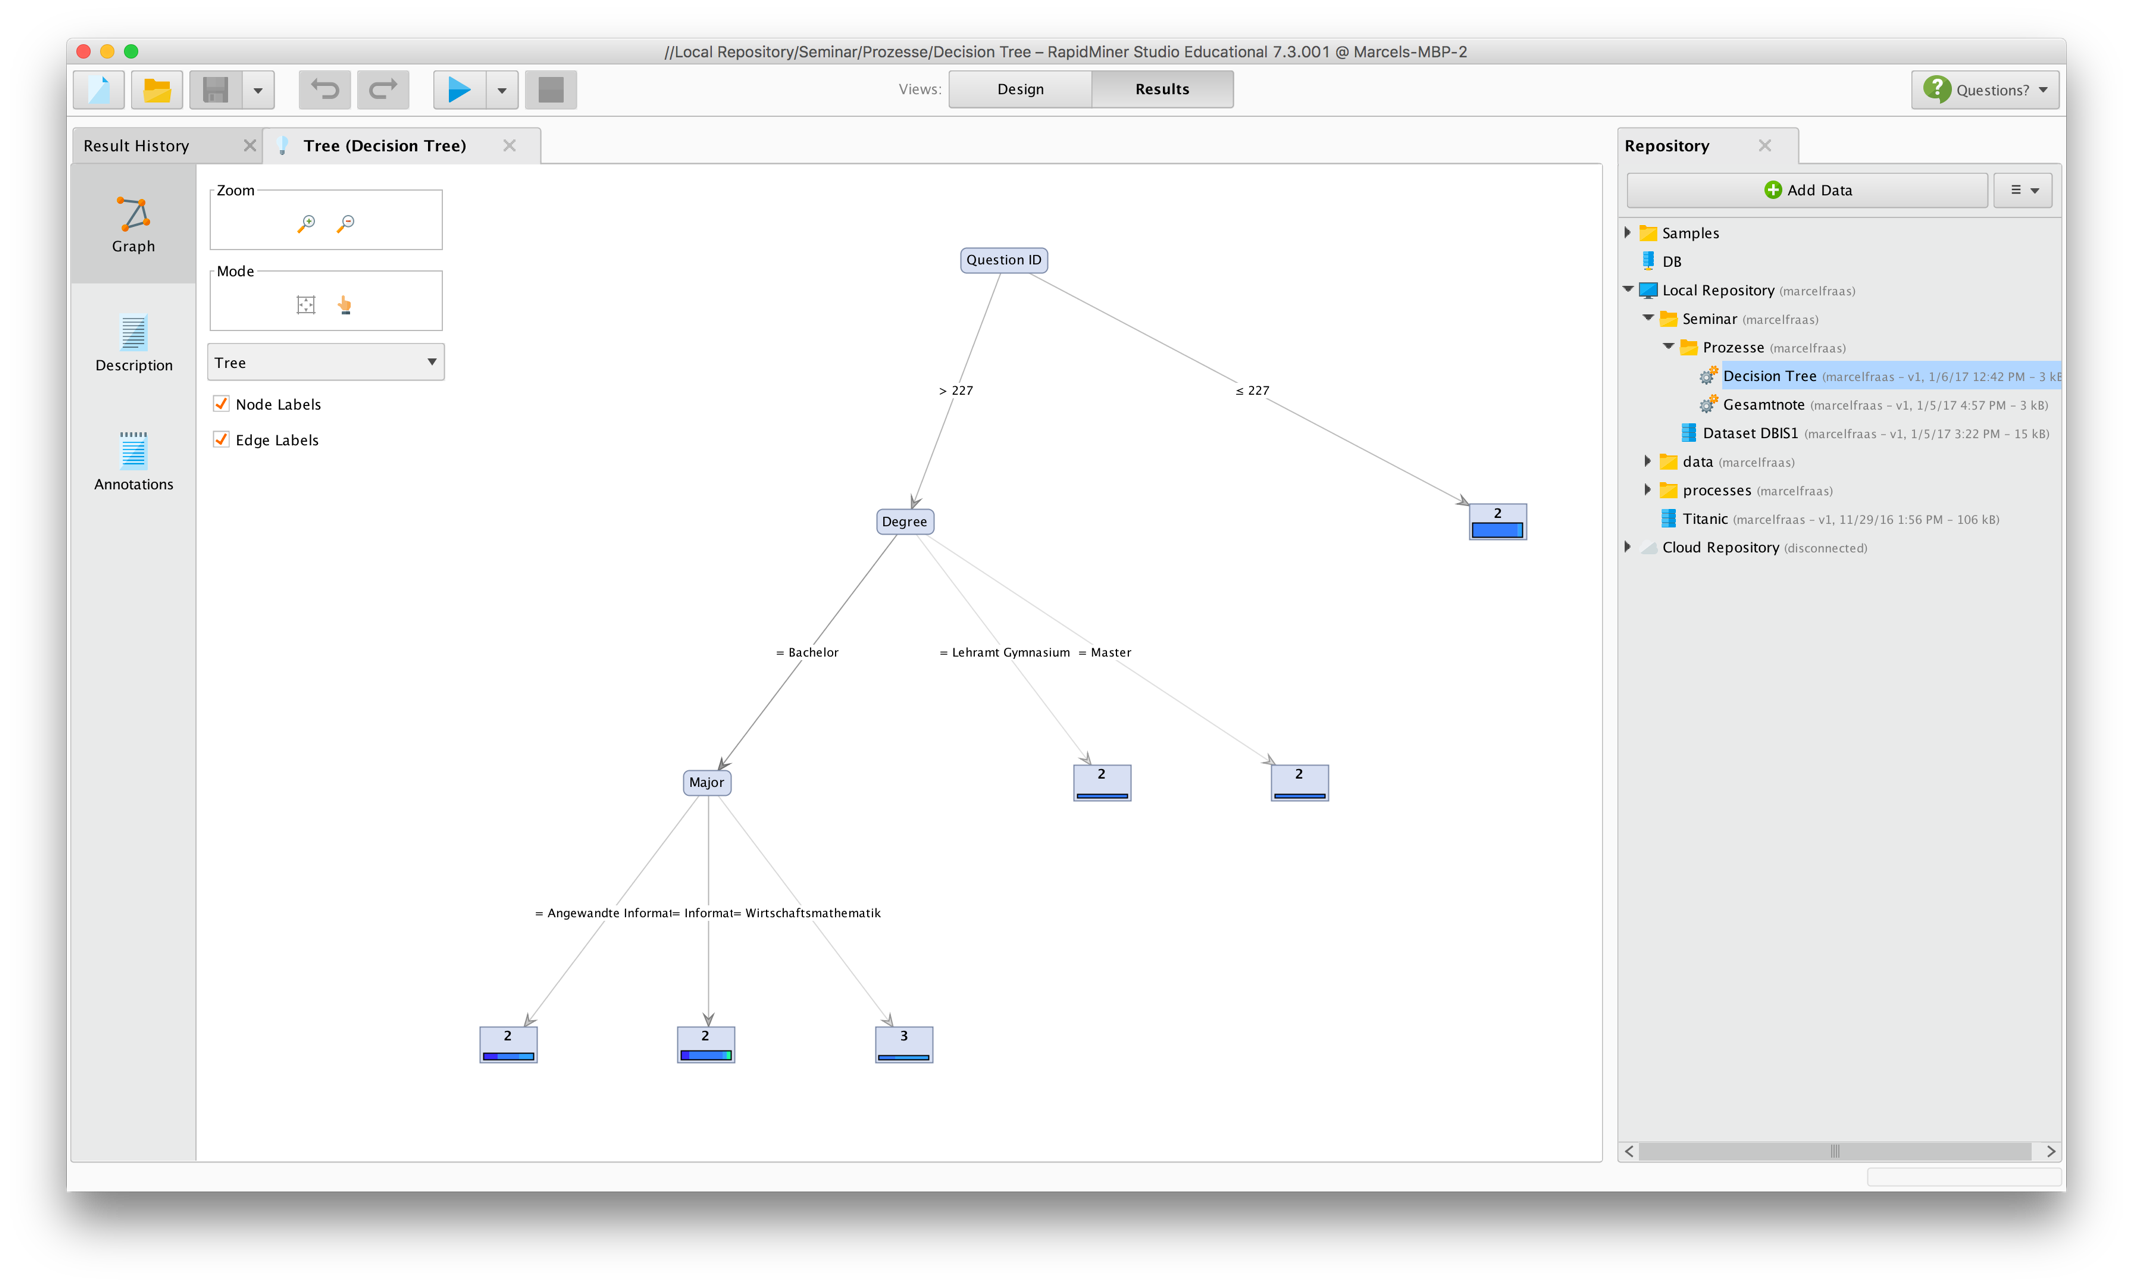
\includegraphics[width=\textwidth]{gfx/rmres.png}
	\caption{Das Ergebnis im RapidMiner Studio}
	\label{fig:example:impl:rm:res}
\end{figure}

Das Ergebnis ist ein Baum, an welchem erkennbar ist, dass in den meisten Fällen
die Note „2“ für die Lehrveranstaltung vergeben wurde. Einzig bei der
Betrachtung des Studienfaches fällt auf, dass Studierende, welche dem „Major“
Wirtschaftsmathematik angehören, eine 3 vergeben haben. An den Blättern lässt
sich außerdem ablesen, wie groß die sog. „Confidence“ ist, also auf wie vielen
Daten, die jeweilige Entscheidung basiert. Kenntlich gemacht wird dies durch
die jeweiligen farblichen Balken. Diese sind wie folgt zu interpretieren: Je
dicker (höher) der Balken, desto mehr Datensätze liegen der Entscheidung
zugrunde. Anhand (der Anzahl) der Farben erkennt man wieviel unterschiedliche
Werte für die jeweilige Klasse gefunden wurden, und entsprechend an der „breite“
der Farbe kann man ablesen, wie oft der jeweilige Wert in Relation aufgetaucht
ist.

\subsection{Microsoft Azure Machine Learning Studio}
\label{sec:example:impl:msa}

Das korrespondierende Experiment im Microsoft Azure Machine Learning Studio
sieht folgendermaßen aus:

\begin{figure}[htb]
  \center
	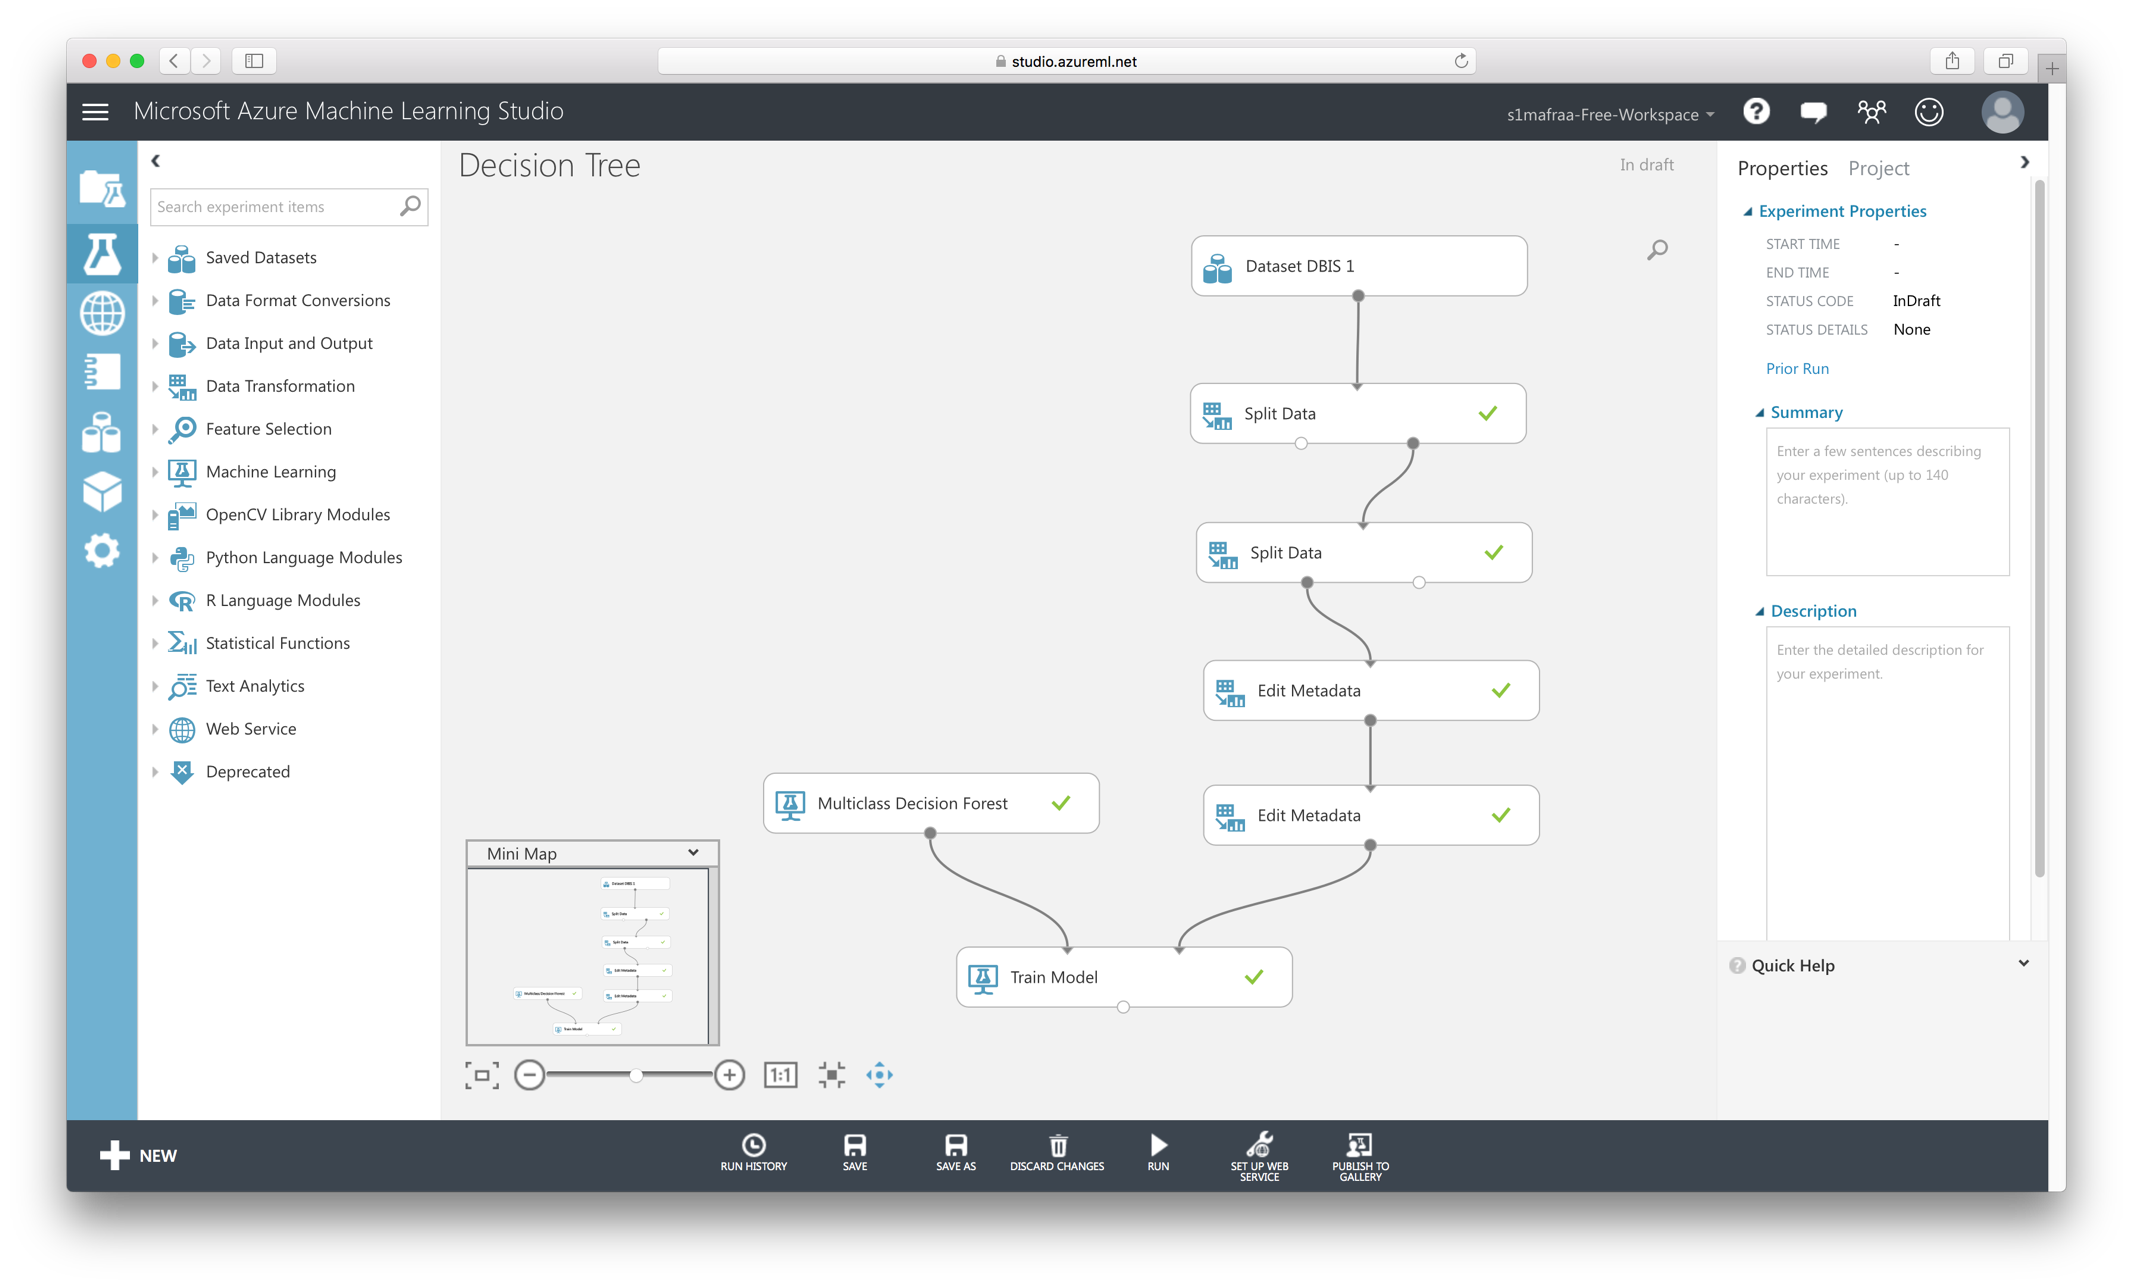
\includegraphics[width=0.85\textwidth]{gfx/msaproc.png}
	\caption{Das Beispiel-Experiment im Microsoft Azure Machine Learning Studio}
	\label{fig:example:impl:msa:proc}
\end{figure}

Hier fällt auf der rechten Seite auf, dass je 2 „Split Data“ und „Edit Metadata“
Operatoren gebraucht wurden. Um die selbe Filter-Funktionalität wie beim
RapidMiner Studio Prozess abzubilden, mussten zunächst alle NULL Einträge und
anschließend ebenfalls alle Datensätze, welche die Frage nach der Gesamtnote
beinhalten, herausgefiltert werden. Dafür waren hier 2 separate „Split“
Operationen notwendig. Des Weiteren wurde sowohl für die Definition des
Attributs „Answer“ als Label, als auch für die Definition der restlichen
Attribute als „klassifizierende Attribute“ je ein „Edit Metadata“ Operator
benötigt. Zuletzt fällt noch auf, dass anstatt eines Decision Tree Algorithmus
ein „Multiclass Decision Forest“, welcher als Konfiguration eine Decision-Tree
Anzahl von 1 bekommen hat, zur Berechnung verwendet wurde. Dies war notwendig,
um überhaupt ein auswertbares Ergebnis zu erhalten, welches zumindest
Ansatzweise mit dem Ergebnis des RapidMiner Studios vergleichbar ist.

\begin{figure}[htb]
  \center
	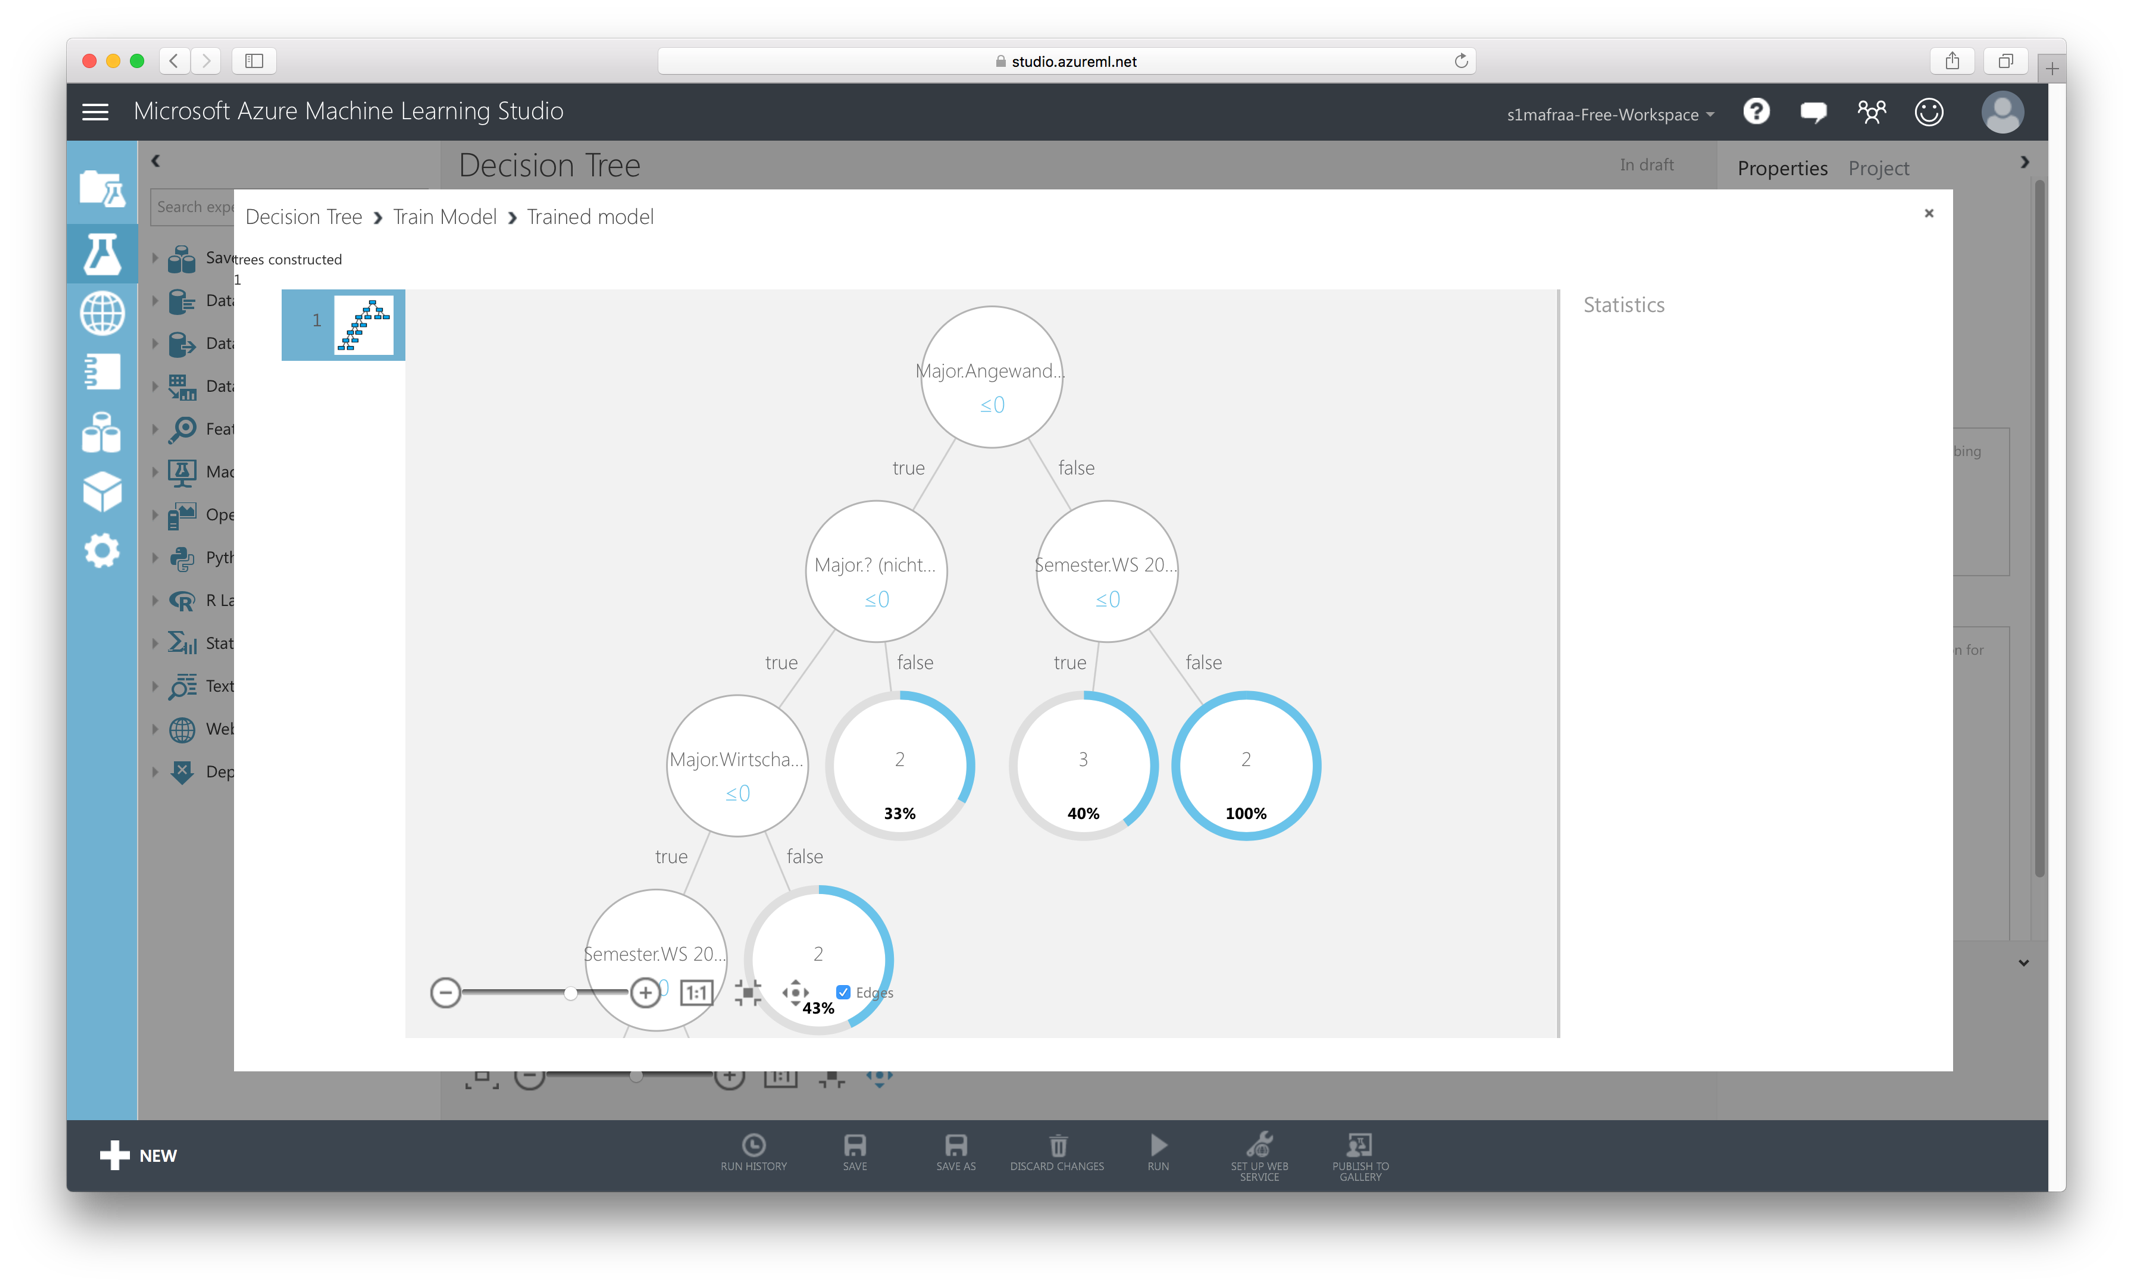
\includegraphics[width=0.85\textwidth]{gfx/msares.png}
	\caption{Das Ergebnis im Microsoft Azure Machine Learning Studio}
	\label{fig:example:impl:msa:res}
\end{figure}

Wie aufgrund der Tatsache, dass ein anderer Algorithmus verwendet wurde,
anzunehmen ist, weicht das Ergebnis vom vorherigen Ergebnis des RapidMiner
Studios in einigen Punkten ab. Der Baum zeigt, dass nicht zwangsläufig das
Studienfach ausschlaggebend für eine schlechtere Bewertung war, sondern das
Semester, in welchem die Umfrage durchgeführt wurde.
Auch hier lässt sich anhand der Blätter ablesen, wie groß die „Confidence“ der
jeweiligen Klasse ist. So lässt sich also interpretieren, dass Studierende, die
nicht dem „Major“ Angewandte Informatik angehören, dafür allerdings im
Wintersemester 2012/13 an der Umfrage teilgenommen haben überwiegend die Note
„3“ vergeben haben. Die Prozentzahl zeigt dabei an, dass 40\% der zugrunde
liegenden Datensätze in die Klasse „3“ fallen, wohingegen die anderen 60\%
sich auf die restlichen Werte 1, 2 bzw. 4, 5 und 6 verteilen.

% !TEX root = ../Seminararbeit-Data_Mining_Frameworks.tex
%


% =============================================================================
%
% Fazit
%
% =============================================================================
\chapter{Fazit}
\label{sec:fazit}

Zum Abschluss werden beide Tools noch einmal in Bezug auf unterschiedliche
Aspekte miteinander verglichen.

\begin{enumerate}
  \item Installation und Setup: \\
  Zunächst konnte das „Setup“ bei beiden Tools ohne Probleme durchgeführt
  werden. Allerdings besitzt das Microsoft Azure Machine Learning Studio
  hier den Vorteil, dass keine Installation (sondern nur eine Registrierung
  bzw. ein Login) notwendig ist und man direkt mit der Analyse seiner Daten
  beginnen kann. Das RapidMiner Studio ist zwar für alle Plattformen erhältlich,
  muss aber dennoch (manuell) installiert werden. Zudem wird eine aktuelle Java
  Runtime vorausgesetzt, welche u.U. auch erst installiert werden muss.
  Microsoft setzt diesbezüglich nur einen (aktuelleren) Internetbrowser voraus.
  \item Features und Funktionen: \\
  Beide Programme kommen mit einer Vielzahl an Implementierungen verschiedener
  Algorithmen. Bezüglich der Anzahl hat das RapidMiner Studio jedoch etwas mehr
  zu bieten.


  \begin{figure}[htb]
    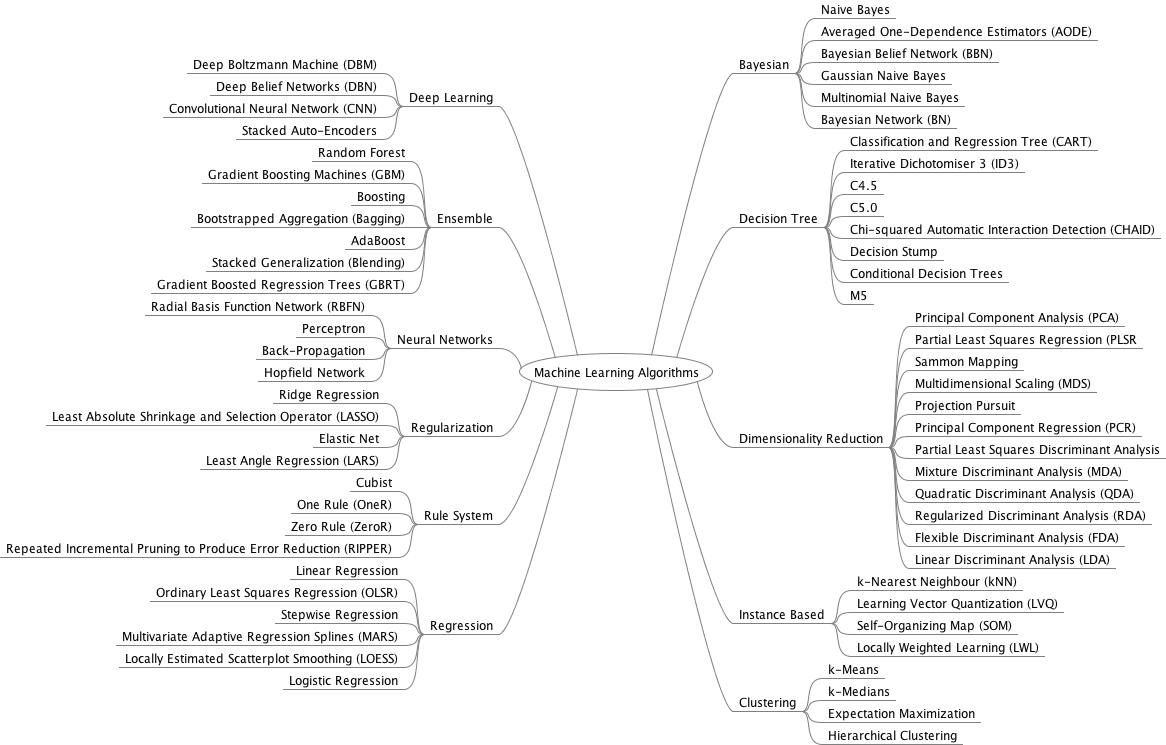
\includegraphics[width=\textwidth]{gfx/rmalgs.png}
    \caption{Algorithmen des RapidMiner Studios \cite{MLM}}
    \label{fig:fazit:rmalgs}
  \end{figure}

  \begin{figure}[htb]
    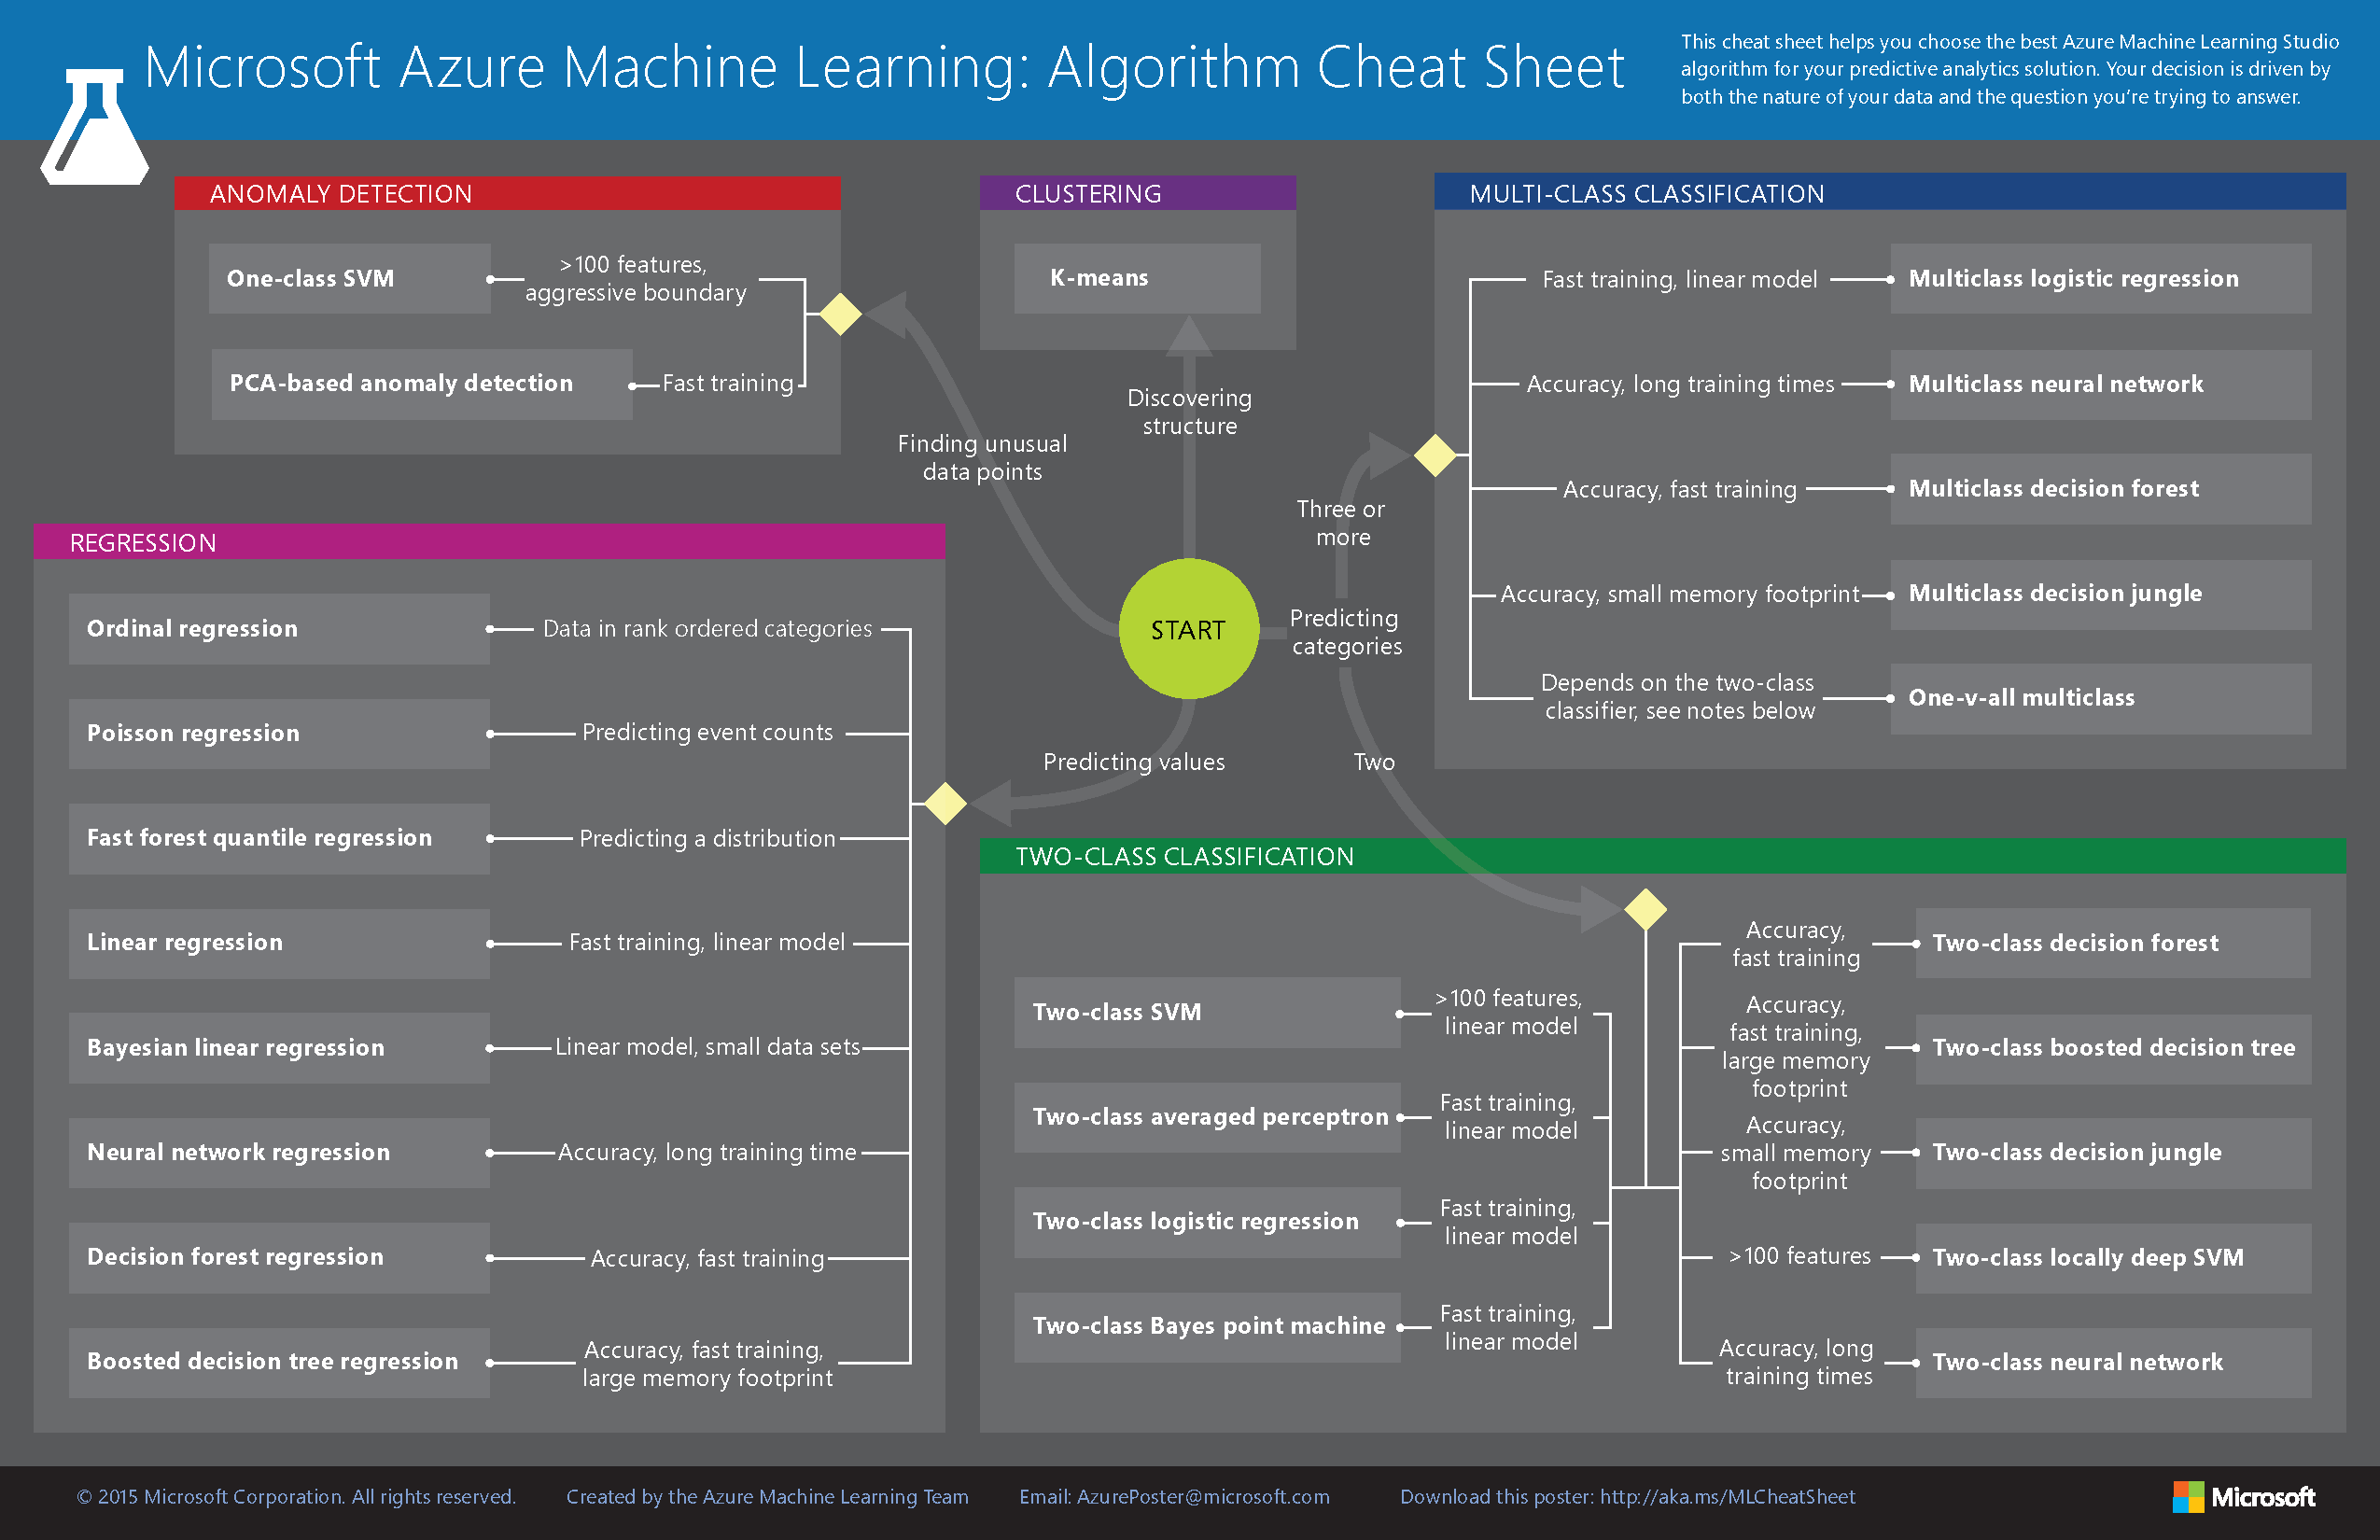
\includegraphics[width=\textwidth]{gfx/msaalgs.pdf}
    \caption{Algorithmen des Microsoft Azure Machine Learning Studios \cite{MSA}}
    \label{fig:fazit:msaalgs}
  \end{figure}
  \item Kollaboration und Zusammenarbeit:
 \\
  Gleiches wie bei der Automatisierung gilt auch für die Unterstützung eines
  kollaborativen Workflows mit mehreren Anwendern. Während in Microsofts
  Machine Learning Studio die Experimente direkt mit anderen Anwendern geteilt
  bzw. zusammen an diesen gearbeitet werden kann, benötigt es auf der RapidMiner
  Plattform eines eigenen Servertools (sofern die Prozesse nicht als Datei
  abgespeichert und per Email verschickt werden wollen).
  \item Bedienung und User Interface: \\
  Bezüglich der Bedienbarkeit bietet das RapidMiner Studio einen angenehm hohen
  Komfort, während das Machine Learning Studio von Microsoft an die
  Webtechnologien und Möglichkeiten eines Internetbrowser gebunden ist. Nichtsdestotrotz
  ist die nötige Einarbeitungszeit bei beiden Tools sehr kurz.
  \item Schnittstellen und Erweiterungsmöglichkeiten: \\
  Da das RapidMiner Studio quelloffen ist, ist es hier möglich, durch Plugins
  die Feature-Liste selbst noch zu erweitern und eigene Algorithmen zu
  implementieren. Jedoch bietet das Microsoft Azure Machine Learning Studio
  hier einen deutlich höheren Komfort, indem es direkt das Einbinden von R
  Skripten, sowie Python Code ermöglicht.
  \item Automatisierung und Deployment
: \\
  Die Experimente können aus dem Machine Learning Studio direkt als
  Webservices exportiert und per REST-API angesteuert werden. Dies ermöglicht
  einen sehr effizienten und schnellen Workflow von der Analyse der Daten hin
  zur Implementierung eines automatisierten Modells in einer bestehenden
  Anwendung. RapidMiner Studio benötigt dagegen für das Deployment einen
  eigene Serverinstallation auf Basis des RapidMiner Servers oder des RapidMiner
  Radoop Tools. Der Administrationsaufwand ist hier daher deutlich höher.
\end{enumerate}

Abschließend lässt sich sagen, dass RapidMiner zurecht die populärere der
beiden Plattformen ist, da diese intuitiver zu bedienen ist und in Sachen
vorgefertigter Algorithmen deutlich mächtiger ist als die Lösung von Microsoft.
Nichtsdestotrotz sollte auch, gerade wenn bereits ein Informationssystem auf
Basis von Microsoft bzw. der Azure Cloud besteht, das Machine Learning Studio
nicht außer Acht gelassen werden.

%% !TEX root = ../Seminararbeit-Data_Mining_Frameworks.tex
%
\chapter{Related Work}
\label{sec:related}

\cleanchapterquote{A picture is worth a thousand words. An interface is worth a thousand pictures.}{Ben Shneiderman}{(Professor for Computer Science)}

\Blindtext[2][1]

\section{Related Work Section 1}
\label{sec:related:sec1}

\Blindtext[2][2]

\section{Related Work Section 2}
\label{sec:related:sec2}

\Blindtext[3][2]

\section{Related Work Section 3}
\label{sec:related:sec3}

\Blindtext[4][2]

\section{Conclusion}
\label{sec:related:conclusion}

\Blindtext[2][1]
 % INCLUDE: related work
%% !TEX root = ../Seminararbeit-Data_Mining_Frameworks.tex
%
\chapter{System}
\label{sec:system}

\cleanchapterquote{Innovation distinguishes between a leader and a follower.}{Steve Jobs}{(CEO Apple Inc.)}

\Blindtext[2][1]

\section{System Section 1}
\label{sec:system:sec1}

\Blindtext[1][2]

\begin{figure}[htb]
	
\includegraphics[width=\textwidth]{gfx/Clean-Thesis-Figure}
	\caption{Figure example: \textit{(a)} example part one, \textit{(c)} example part two; \textit{(c)} example part three}
	\label{fig:system:example1}
\end{figure}

\Blindtext[1][2]

\section{System Section 2}
\label{sec:system:sec2}

\Blindtext[1][2]

\begin{figure}[htb]
	
\includegraphics[width=\textwidth]{gfx/Clean-Thesis-Figure}
	\caption{Another Figure example: \textit{(a)} example part one, \textit{(c)} example part two; \textit{(c)} example part three}
	\label{fig:system:example2}
\end{figure}

\Blindtext[2][2]

\section{System Section 3}
\label{sec:system:sec3}

\Blindtext[4][2]

\section{Conclusion}
\label{sec:system:conclusion}

\Blindtext[2][1]
	% INCLUDE: system
%% !TEX root = ../Seminararbeit-Data_Mining_Frameworks.tex
%
\chapter{Concepts}
\label{sec:concepts}

\cleanchapterquote{Users do not care about what is inside the box, as long as the box does what they need done.}{Jef Raskin}{about Human Computer Interfaces}

\Blindtext[2][1]

\section{Concepts Section 1}
\label{sec:concepts:sec1}

\Blindtext[2][2]

\section{Concepts Section 2}
\label{sec:concepts:sec2}

\Blindtext[3][2]

\section{Concepts Section 3}
\label{sec:concepts:sec3}

\Blindtext[4][2]

\section{Conclusion}
\label{sec:concepts:conclusion}

\Blindtext[2][1]
 % INCLUDE: concepts
%% !TEX root = ../Seminararbeit-Data_Mining_Frameworks.tex
%
\chapter{Conclusion}
\label{sec:conclusion}

\Blindtext[2][1]

\section{System Section 1}
\label{sec:conclusion:sec1}

\Blindtext[2][2]

\section{System Section 2}
\label{sec:conclusion:sec2}

\Blindtext[3][2]

\section{Future Work}
\label{sec:conclusion:future}

\Blindtext[2][2]
 % INCLUDE: conclusion
\cleardoublepage

% --------------------------
% Back matter
% --------------------------
{%
\setstretch{1.1}
\renewcommand{\bibfont}{\normalfont\small}
\setlength{\biblabelsep}{0pt}
\setlength{\bibitemsep}{0.5\baselineskip plus 0.5\baselineskip}
\printbibliography[nottype=online]
\printbibliography[heading=subbibliography,title={Websites},type=online,prefixnumbers={@}]
}
\cleardoublepage

\listoffigures
\cleardoublepage

%\listoftables
%\cleardoublepage

%% !TEX root = ../Seminararbeit-Data_Mining_Frameworks.tex
%
%************************************************
% Declaration
%************************************************
\pdfbookmark[0]{Declaration}{Declaration}
\chapter*{Declaration}
\label{sec:declaration}
\thispagestyle{empty}

You can put your declaration here, to declare that you have completed your work solely and only with the help of the references you mentioned.

\bigskip

\noindent\textit{\thesisUniversityCity, \thesisDate}

\smallskip

\begin{flushright}
	\begin{minipage}{5cm}
		\rule{\textwidth}{1pt}
		\centering\thesisName
	\end{minipage}
\end{flushright}

%*****************************************
%*****************************************

\clearpage
\newpage
\mbox{}

% **************************************************
% End of Document CONTENT
% **************************************************
\end{document}
